\documentclass[12pt,a4paper]{article}
\usepackage[a4paper, margin=0.8in, headheight=14pt]{geometry}
\usepackage{fontspec}
\usepackage{unicode-math}
\setmainfont{TeX Gyre Pagella}
\setmonofont[Scale=0.88]{TeX Gyre Cursor}
\setmathfont{Latin Modern Math}
\usepackage{xcolor}
\usepackage{colortbl}
\usepackage{titlesec}
\usepackage{enumitem}
\usepackage{tabularx}
\usepackage{booktabs}
\usepackage{array}
\usepackage{amsmath}
\usepackage{tikz}
\usetikzlibrary{shapes.geometric, arrows.meta, positioning, calc, fit, decorations.pathreplacing, decorations.pathmorphing}
\usepackage{tcolorbox}
\tcbuselibrary{skins, breakable}
\usepackage{hyperref}
\usepackage{fancyhdr}
\usepackage{graphicx}
\usepackage{microtype}
\hyphenpenalty=10000
\exhyphenpenalty=10000
\sloppy
\usepackage{caption}
\usepackage{setspace}
\usepackage{multirow}
\usepackage{tocloft}
\newcommand{\Q}[1]{\textbf{#1}\par\noindent\ignorespaces}
\definecolor{myred}{RGB}{196,30,58}
\definecolor{mydark}{RGB}{30,30,50}
\definecolor{mygreen}{RGB}{14,120,80}
\definecolor{myteal}{RGB}{0,130,140}
\definecolor{myamber}{RGB}{180,100,0}
\definecolor{mypurple}{RGB}{100,30,160}
\definecolor{mygray}{RGB}{246,247,249}
\definecolor{mgframe}{RGB}{180,185,200}
\definecolor{watermark}{RGB}{145,150,170}
\definecolor{hdrred}{RGB}{250,232,235}
\definecolor{hdrgreen}{RGB}{220,244,233}
\definecolor{hdrteal}{RGB}{220,242,244}
\definecolor{hdramber}{RGB}{253,242,215}
\definecolor{hdrpurple}{RGB}{238,228,255}
\definecolor{hdrgray}{RGB}{238,240,245}
\definecolor{rowalt}{RGB}{250,251,253}

\titleformat{\section}{\large\bfseries\color{myred}}{\thesection.}{0.5em}{}[\vspace{1pt}{\color{myred}\rule{\linewidth}{0.8pt}}]
\titleformat{\subsection}{\normalsize\bfseries\color{myteal}}{\thesubsection}{0.5em}{}
\titlespacing*{\section}{0pt}{18pt}{7pt}
\titlespacing*{\subsection}{0pt}{11pt}{4pt}
\setlength{\parindent}{0pt}
\setlength{\parskip}{4pt}
\renewcommand{\cfttoctitlefont}{\large\bfseries\color{myred}}
\renewcommand{\cftaftertoctitle}{\par\noindent{\color{myred}\rule{\linewidth}{0.8pt}}}
\setlength{\cftbeforetoctitleskip}{0pt}
\setlength{\cftaftertoctitleskip}{6pt}
\renewcommand{\cftsecfont}{\normalsize\bfseries\color{mydark}}
\renewcommand{\cftsecpagefont}{\normalsize\bfseries\color{mydark}}
\renewcommand{\cftsecleader}{\cftdotfill{\cftdotsep}}
\setlength{\cftbeforesecskip}{7pt}
\renewcommand{\cftsubsecfont}{\small\color{mydark}}
\renewcommand{\cftsubsecpagefont}{\small\color{mydark}}
\setlength{\cftbeforesubsecskip}{3pt}
\setlength{\cftsubsecindent}{1.4em}
\renewcommand{\cftpartfont}{\normalsize\bfseries\color{myteal}}
\renewcommand{\cftpartpagefont}{\normalsize\bfseries\color{myteal}}
\setlength{\cftbeforepartskip}{14pt}
\renewcommand{\arraystretch}{1.45}
\setlength{\tabcolsep}{6pt}
\arrayrulecolor{mydark}
\newcolumntype{B}[1]{>{\small\bfseries\raggedright\arraybackslash}m{#1}}
\newcolumntype{C}[1]{>{\centering\arraybackslash}m{#1}}
\newcolumntype{Y}{>{\small\raggedright\arraybackslash}X}
\renewcommand{\tabularxcolumn}[1]{m{#1}}
\newcommand{\currmodule}{Module 1}
\pagestyle{fancy}
\fancyhf{}
\fancyhead[L]{\small\color{myred}\textbf{PE-EC703B}\;\color{mydark}--- Wireless Sensor Networks}
\fancyhead[R]{\small\color{myteal}\textbf{\currmodule\ Notes}}
\fancyfoot[C]{\small\color{mydark}\thepage}
\fancyfoot[R]{\small\color{watermark}\textit{\copyright\ Biraj}}
\renewcommand{\headrulewidth}{0.5pt}
\renewcommand{\footrulewidth}{0.3pt}

\hypersetup{colorlinks=true, linkcolor=myteal, urlcolor=myteal,
  pdfauthor={Biraj Sarkar},
  pdftitle={PE-EC703B --- Combined Notes}}

\tcbset{
  tikzbox/.style={
    colback=mygray, colframe=mgframe, boxrule=0.6pt, arc=4pt,
    left=8pt, right=8pt, top=6pt, bottom=6pt,
    colbacktitle=mgframe, coltitle=mydark,
    fonttitle=\small\bfseries
  },
  defbox/.style={
    colback=hdrgreen, colframe=mygreen, boxrule=0.8pt, arc=4pt,
    left=9pt, right=9pt, top=6pt, bottom=6pt,
    colbacktitle=mygreen, coltitle=white,
    fonttitle=\small\bfseries
  },
  formulabox/.style={
    colback=hdrteal, colframe=myteal, boxrule=0.8pt, arc=4pt,
    left=9pt, right=9pt, top=7pt, bottom=7pt,
    colbacktitle=myteal, coltitle=white,
    fonttitle=\small\bfseries
  },
  examplebox/.style={
    colback=hdramber, colframe=myamber, boxrule=0.8pt, arc=4pt,
    left=9pt, right=9pt, top=6pt, bottom=6pt,
    colbacktitle=myamber, coltitle=white,
    fonttitle=\small\bfseries
  },
  masonbox/.style={
    colback=hdrpurple, colframe=mypurple, boxrule=0.8pt, arc=4pt,
    left=9pt, right=9pt, top=6pt, bottom=6pt,
    colbacktitle=mypurple, coltitle=white,
    fonttitle=\small\bfseries
  },
  exambox/.style={
    colback=hdrpurple, colframe=mypurple, boxrule=1pt, arc=5pt,
    left=10pt, right=10pt, top=8pt, bottom=8pt,
    colbacktitle=mypurple, coltitle=white,
    fonttitle=\bfseries,
    breakable, title after break={\textbf{Frequently Asked / Viva Questions (contd.)}}}
}
\tcbset{breakable}
\tcbset{after={\color{black}}}

\tikzset{
  block/.style={rectangle, draw=myteal, fill=hdrteal,
    text width=2.4cm, align=center, minimum height=0.95cm,
    font=\small, rounded corners=3pt, line width=0.7pt},
  redblock/.style={rectangle, draw=myred, fill=hdrred,
    text width=2.4cm, align=center, minimum height=0.95cm,
    font=\small, rounded corners=3pt, line width=0.7pt},
  netnode/.style={rectangle, draw=myteal, fill=hdrteal,
    text width=1.5cm, align=center, minimum height=0.8cm,
    font=\small, rounded corners=3pt, line width=0.7pt},
  sumjunc/.style={circle, draw=myamber, fill=hdramber,
    minimum size=0.62cm, font=\small, line width=0.8pt},
  snode/.style={circle, draw=mypurple, fill=hdrpurple,
    minimum size=0.55cm, font=\footnotesize, line width=0.7pt},
  arrow/.style={-Stealth, thick, color=mydark},
  redarrow/.style={-Stealth, thick, color=myred},
  line/.style={thick, color=mydark}
}

\newcommand{\modulestart}[2]{%
  \clearpage
  \renewcommand{\currmodule}{Module #1}%
  \phantomsection
  \addcontentsline{toc}{part}{Module #1: #2}%
  \setcounter{section}{0}%
  \begin{center}
    \vspace*{1.0cm}
    {\Huge\bfseries\color{myred} Module #1}\\[10pt]
    {\Large\bfseries\color{mydark} #2}\\[10pt]
    {\color{myred}\rule{0.55\linewidth}{1.2pt}}
  \end{center}
  \vspace{14pt}
}
\begin{document}

\thispagestyle{empty}
\vspace*{1.0cm}
\begin{center}
  {\Huge\bfseries\color{myred} PE-EC703B}\\[10pt]
  {\LARGE\bfseries\color{mydark} Wireless Sensor Networks}\\[20pt]
  {\color{myred}\rule{0.7\linewidth}{1.5pt}}\\[18pt]
  {\Large\color{myteal}\textbf{Combined Module Notes}}\\[8pt]
  {\large\color{mydark} Modules 1 -- 5}\\[40pt]
  {\normalsize\color{mydark} Semester VII \quad$\bullet$\quad 3L:0T:0P \quad$\bullet$\quad 3 Credits}\\[12pt]
  {\normalsize\color{mydark} CGEC \;$|$\; B.Tech ECE (2023--27)}\\[6pt]
  {\normalsize\color{mydark}\textit{Biraj Sarkar}}
\end{center}
\vspace{1.0cm}
\begin{center}
  \begin{tcolorbox}[colback=mygray, colframe=mgframe, boxrule=0.5pt, arc=3pt, width=0.85\linewidth]
    \centering\small\color{mydark}
    \textbf{Disclaimer / Study Guide Notice:}\\
    These are condensed \textbf{Short Notes} focusing on core theory, key formulas, block/circuit diagrams, and standard viva Q\&As for university exam revision. Exhaustive numerical practice problems and derivation edge cases are not covered. This serves as a quick-revision reference guide for students.
  \end{tcolorbox}
\end{center}
\vfill
\begin{center}{\small\color{watermark}\textit{Exam-Ready Notes}}\end{center}
\clearpage

\hypersetup{linkcolor=mydark}
\tableofcontents
\hypersetup{linkcolor=myteal}
\clearpage

% -- Module 1 -----------------------------------------------------------------
\modulestart{1}{What is a Wireless Sensor Network?}

\section{What is a Wireless Sensor Network?}
% ===============================================================================

A Wireless Sensor Network (WSN) is a distributed network of small, low-power sensor nodes that are spatially deployed to monitor physical or environmental conditions and cooperatively communicate data to a central point (sink or base station).

\begin{tcolorbox}[defbox, title={\textbf{Wireless Sensor Network (WSN) --- Definition}}]
A \textbf{Wireless Sensor Network} is a self-organizing collection of spatially distributed, resource-constrained sensor nodes that sense physical parameters (temperature, pressure, motion, light, etc.) and transmit collected data wirelessly, usually through multi-hop communication, to a \textbf{sink node} or \textbf{base station} for processing and action.
\end{tcolorbox}

A WSN consists of:
\begin{itemize}[leftmargin=*, itemsep=3pt]
  \item \textbf{Sensor nodes (motes):} Battery-powered miniature devices with sensing, processing, and wireless communication capability.
  \item \textbf{Sink node (base station):} Aggregates all data from sensor nodes and forwards to an external network or user.
  \item \textbf{Task manager node:} Issues tasks (queries) into the network and receives aggregated results.
  \item \textbf{Communication medium:} Wireless radio (IEEE 802.15.4, ZigBee, Bluetooth LE).
\end{itemize}

\begin{tcolorbox}[tikzbox, title={WSN Architecture --- Sensing Field to User}]
\centering
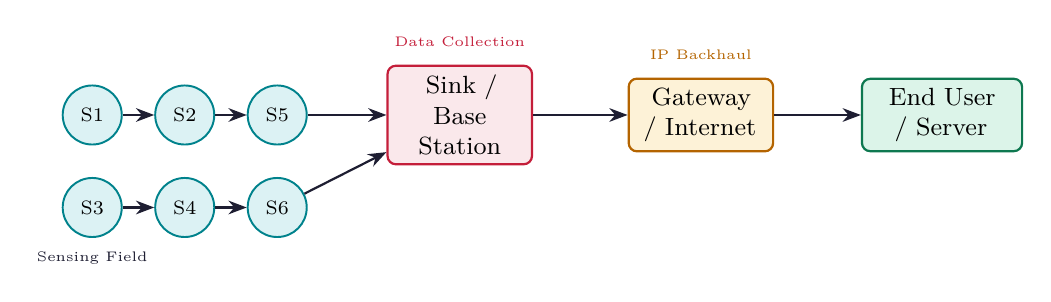
\begin{tikzpicture}[node distance=0.5cm and 1.1cm,
  wsnode/.style={circle, draw=myteal, fill=hdrteal, minimum size=0.75cm, font=\scriptsize, align=center, line width=0.7pt},
  sinknode/.style={rectangle, draw=myred, fill=hdrred, text width=1.6cm, align=center, minimum height=0.85cm, font=\small, rounded corners=3pt, line width=0.8pt},
  gwnode/.style={rectangle, draw=myamber, fill=hdramber, text width=1.6cm, align=center, minimum height=0.85cm, font=\small, rounded corners=3pt, line width=0.8pt},
  usernode/.style={rectangle, draw=mygreen, fill=hdrgreen, text width=1.8cm, align=center, minimum height=0.85cm, font=\small, rounded corners=3pt, line width=0.8pt}]

  % Sensor nodes
  \node[wsnode] (n1) {S1};
  \node[wsnode, right=0.4cm of n1] (n2) {S2};
  \node[wsnode, below=0.4cm of n1] (n3) {S3};
  \node[wsnode, right=0.4cm of n3] (n4) {S4};
  \node[wsnode, right=0.4cm of n2] (n5) {S5};
  \node[wsnode, right=0.4cm of n4] (n6) {S6};

  % Sink
  \node[sinknode, right=1.0cm of n5] (sink) {Sink / Base Station};

  % Gateway
  \node[gwnode, right=1.2cm of sink] (gw) {Gateway / Internet};

  % User
  \node[usernode, right=1.1cm of gw] (usr) {End User / Server};

  % Arrows: sensor to sensor (multi-hop)
  \draw[arrow] (n1) -- (n2);
  \draw[arrow] (n3) -- (n4);
  \draw[arrow] (n2) -- (n5);
  \draw[arrow] (n4) -- (n6);
  \draw[arrow] (n5) -- (sink);
  \draw[arrow] (n6) -- (sink);
  \draw[arrow] (sink) -- (gw);
  \draw[arrow] (gw) -- (usr);

  % Labels
  \node[font=\tiny, color=mydark, below=0.05cm of n3] {Sensing Field};
  \node[font=\tiny, color=myred, above=0.1cm of sink] {Data Collection};
  \node[font=\tiny, color=myamber, above=0.1cm of gw] {IP Backhaul};
\end{tikzpicture}
\end{tcolorbox}

% ===============================================================================
\section{Unique Constraints and Challenges in WSN}
% ===============================================================================

WSNs operate under severe resource limitations that do not apply to traditional networks. These constraints fundamentally drive the design of every protocol and algorithm in WSN.

\subsection{Unique Constraints}

\begin{tcolorbox}[formulabox, title={\textbf{Key Constraints of WSN}}]
\begin{enumerate}[leftmargin=*, itemsep=4pt]
  \item \textbf{Energy constraint:} Sensor nodes are battery-powered with limited energy. Replacing batteries is often impractical (nodes deployed in remote or harsh environments). Energy governs node lifetime and hence network lifetime.
  \item \textbf{Computation constraint:} Nodes have very limited processing power (e.g., 8-bit or 16-bit microcontrollers at 4--16 MHz). Complex algorithms cannot run on-node.
  \item \textbf{Memory constraint:} Typically only 4--10 KB RAM and 48--256 KB flash. Large routing tables or data buffers are infeasible.
  \item \textbf{Communication constraint:} Short-range radio (10--100 m), low bandwidth (20--250 kbps), high bit-error rates, and half-duplex operation.
  \item \textbf{Physical size constraint:} Nodes must be very small (mote form factor); this restricts antenna size, battery capacity, and sensor quality.
  \item \textbf{Cost constraint:} Mass deployment requires nodes to be cheap (Rs.~100--2000 per node). This limits hardware quality.
\end{enumerate}
\end{tcolorbox}

\subsection{Challenges}

\begin{itemize}[leftmargin=*, itemsep=3pt]
  \item \textbf{Scalability:} Networks may contain hundreds to thousands of nodes. Protocols must scale without central control.
  \item \textbf{Fault tolerance:} Nodes fail due to battery depletion or physical damage. The network must self-heal and reroute.
  \item \textbf{Dynamic topology:} Nodes may join, leave, or move; links break frequently. Routing must adapt dynamically.
  \item \textbf{Data-centric communication:} Unlike address-centric IP networks, WSN queries are about \emph{what} data (e.g., ``temperature $> 50$°C''), not \emph{where} a node is.
  \item \textbf{Localization:} Knowing the geographic position of a node is essential for many applications but GPS is expensive and power-hungry.
  \item \textbf{Synchronization:} Nodes need time-synchronized sleep/wake cycles; clocks drift over time.
  \item \textbf{Security:} Nodes operate in hostile environments; attackers can eavesdrop, inject, or jam communications.
  \item \textbf{QoS:} Latency, reliability, and data freshness requirements vary by application.
\end{itemize}

% ===============================================================================
\section{Advantages of Sensor Networks}
% ===============================================================================

\begin{tcolorbox}[examplebox, title={\textbf{Why Use WSNs? --- Key Advantages}}]
\begin{itemize}[leftmargin=*, itemsep=4pt]
  \item \textbf{Infrastructure-free deployment:} No cables or fixed infrastructure needed. Nodes can be air-dropped or scattered over terrain.
  \item \textbf{Dense spatial coverage:} Hundreds of nodes provide granular, distributed sensing impossible with a single instrument.
  \item \textbf{Real-time monitoring:} Continuous data collection and event detection without human presence.
  \item \textbf{Self-organizing:} Nodes autonomously form a network, discover neighbors, and elect cluster heads.
  \item \textbf{Fault tolerance:} Redundant nodes maintain coverage even when individual nodes fail.
  \item \textbf{Cost-effective:} Mass production makes per-node cost very low; no installation labor needed.
  \item \textbf{Accessibility:} Can operate in hazardous, remote, or physically inaccessible environments (volcanoes, battlefields, pipelines).
  \item \textbf{Long-term monitoring:} With proper sleep scheduling, networks can last months to years.
\end{itemize}
\end{tcolorbox}

% ===============================================================================
\section{Applications of Sensor Networks}
% ===============================================================================

WSNs are used across virtually every domain requiring unattended, distributed data collection.

\par\noindent
{\renewcommand{\arraystretch}{1.5}%
\begin{tabularx}{\linewidth}{|B{3.0cm}|Y|Y|}
\hline
\textbf{Domain} & \textbf{Application} & \textbf{Parameters Sensed} \\
\hline
\textbf{Military} & Battlefield surveillance, intrusion detection, target tracking & Motion, acoustic, seismic \\
\hline
\textbf{Environment} & Forest fire detection, flood monitoring, wildlife tracking & Temperature, humidity, CO$_2$, water level \\
\hline
\textbf{Health / Medical} & Patient monitoring, assisted living, drug delivery & Heart rate, blood pressure, glucose, posture \\
\hline
\textbf{Industrial} & Machine condition monitoring, pipeline leak detection, factory automation & Vibration, pressure, flow, temperature \\
\hline
\textbf{Agriculture} & Precision farming, soil moisture, irrigation control & Soil pH, moisture, light, temperature \\
\hline
\textbf{Smart Home} & Appliance control, security, energy management & Light, motion, temperature, CO levels \\
\hline
\textbf{Infrastructure} & Structural health monitoring of bridges, buildings & Strain, vibration, tilt, displacement \\
\hline
\textbf{Transportation} & Vehicle detection, traffic management, parking & Magnetic, acoustic, optical \\
\hline
\end{tabularx}}

% ===============================================================================
\section{Types of Wireless Sensor Networks}
% ===============================================================================

WSNs are classified based on deployment medium, node mobility, and communication model.

\subsection{Based on Deployment Medium}

\par\noindent
{\renewcommand{\arraystretch}{1.5}%
\begin{tabularx}{\linewidth}{|B{3.2cm}|Y|Y|}
\hline
\textbf{Type} & \textbf{Description} & \textbf{Applications} \\
\hline
\textbf{Terrestrial WSN} & Nodes deployed on land; communicate via ground-level radio; most common type & Environmental monitoring, agriculture, smart cities \\
\hline
\textbf{Underground WSN} & Nodes buried in soil; signals travel through earth; high attenuation; expensive & Pipeline monitoring, precision agriculture \\
\hline
\textbf{Underwater WSN} & Nodes deployed in water; use acoustic communication (RF attenuates rapidly in water); low bandwidth, high delay & Oceanographic data collection, pollution detection \\
\hline
\textbf{Multimedia WSN} & Nodes equipped with cameras, microphones; high data rate; large bandwidth demand & Surveillance, traffic monitoring \\
\hline
\textbf{Mobile WSN} & Nodes can move (mobile robots, vehicles); topology changes dynamically; harder routing & Target tracking, disaster response \\
\hline
\end{tabularx}}

\subsection{Based on Network Topology}

\begin{itemize}[leftmargin=*, itemsep=3pt]
  \item \textbf{Star topology:} All nodes communicate directly with the base station. Simple but range-limited.
  \item \textbf{Mesh topology:} Multi-hop communication; nodes relay each other's data. Scalable and fault-tolerant.
  \item \textbf{Cluster topology (hierarchical):} Nodes are grouped into clusters with a cluster head (CH) that aggregates data and relays to base station. Energy-efficient; used in LEACH protocol.
  \item \textbf{Tree topology:} Data flows from leaves to root (base station) along a routing tree. Efficient but vulnerable to root-link failures.
\end{itemize}

\subsection{WSN vs. Traditional Wireless Network}

\par\noindent
{\renewcommand{\arraystretch}{1.5}%
\begin{tabularx}{\linewidth}{|B{3.2cm}|Y|Y|}
\hline
\textbf{Parameter} & \textbf{WSN} & \textbf{Traditional Wireless (Wi-Fi/cellular)} \\
\hline
\textbf{Node count} & 10s to 1000s of nodes & Few to dozens of clients \\
\hline
\textbf{Energy} & Battery-powered, must last months/years & Rechargeable or mains-powered \\
\hline
\textbf{Data rate} & Very low (kbps) & High (Mbps -- Gbps) \\
\hline
\textbf{Addressing} & Data-centric (attribute-based) & Address-centric (IP-based) \\
\hline
\textbf{Deployment} & Dense, unattended, random & Planned, maintained \\
\hline
\textbf{Topology} & Dynamic, self-organizing & Mostly static (infrastructure mode) \\
\hline
\textbf{Reliability} & Node failure expected; redundancy built-in & Individual node failure is exceptional \\
\hline
\textbf{Cost per node} & Very low (Rs.~100--2000) & Moderate to high \\
\hline
\end{tabularx}}

% ===============================================================================
\newpage
\section{Quick Revision --- Module 1}
% ===============================================================================

\begin{tcolorbox}[formulabox, title={\textbf{Key Formulas and Metrics at a Glance}}]
\begin{itemize}[leftmargin=*, itemsep=4pt]
  \item \textbf{Network Lifetime} = Time until the first node (or $k$-th node) exhausts its energy.
  \item \textbf{Energy budget per node:} $E_{\text{total}} = E_{\text{sense}} + E_{\text{process}} + E_{\text{tx}} + E_{\text{rx}}$
  \item \textbf{Tx energy model:} $E_{tx}(l, d) = l \cdot E_{\text{elec}} + l \cdot \varepsilon_{\text{amp}} \cdot d^n$ \quad ($n=2$ free space, $n=4$ multipath)
  \item \textbf{Rx energy model:} $E_{rx}(l) = l \cdot E_{\text{elec}}$
  \item \textbf{Coverage:} Area monitored per node $= \pi r_s^2$, where $r_s$ is sensing radius.
  \item \textbf{Connectivity radius:} $r_c \geq r_s$ for a connected network (typically $r_c \approx 2r_s$).
\end{itemize}
\end{tcolorbox}

\begin{tcolorbox}[defbox, title={\textbf{One-Line Definitions}}]
\begin{itemize}[leftmargin=*, itemsep=3pt]
  \item \textbf{WSN:} A distributed system of sensor nodes that sense, process, and wirelessly communicate environmental data to a sink.
  \item \textbf{Sensor node (mote):} A resource-constrained device with sensing, processing, communication, and power units.
  \item \textbf{Sink node:} The data collection point of a WSN; gateway between sensor network and external network.
  \item \textbf{Cluster head (CH):} An elected node that aggregates data from its cluster members and forwards it to the base station.
  \item \textbf{Multi-hop routing:} Technique where data is relayed node-by-node across the network to the sink.
  \item \textbf{Data aggregation:} Combining data from multiple nodes into a single message to reduce redundancy and save energy.
  \item \textbf{Terrestrial WSN:} Nodes deployed on land surface; most common WSN type.
  \item \textbf{Underwater WSN:} Uses acoustic communication because RF signals attenuate rapidly in water.
\end{itemize}
\end{tcolorbox}

\begin{tcolorbox}[exambox, title={\textbf{Frequently Asked / Viva Questions --- Module 1}}]
\begin{enumerate}[leftmargin=*, itemsep=5pt]
  \item \Q{What is a Wireless Sensor Network? How does it differ from a traditional wireless network?}
  A WSN is a distributed network of battery-powered, resource-constrained sensor nodes that sense physical parameters and communicate data wirelessly to a sink. Key differences: WSN is data-centric, has very low power budgets, nodes may fail, and topology is self-organizing, unlike address-centric, infrastructure-based traditional networks.

  \item \Q{What are the unique constraints of WSN?}
  The six key constraints are: (1) \textbf{Energy} --- limited battery, hardest to replace; (2) \textbf{Computation} --- low-speed MCU; (3) \textbf{Memory} --- few KB RAM; (4) \textbf{Communication} --- short range, low bandwidth; (5) \textbf{Size} --- mote form factor; (6) \textbf{Cost} --- mass deployment mandates cheap nodes.

  \item \Q{Why is energy the most critical constraint in WSN?}
  Sensor nodes are battery-powered and often deployed in inaccessible locations (forests, pipelines, battlefields) where battery replacement is impractical. Once energy is exhausted, the node dies, reducing coverage and potentially disconnecting the network. Energy directly determines network lifetime.

  \item \Q{Name and explain three types of WSN based on deployment medium.}
  (1) \textbf{Terrestrial WSN} --- nodes on land, RF communication, most common. (2) \textbf{Underwater WSN} --- uses acoustic signals since RF attenuates in water; low bandwidth. (3) \textbf{Underground WSN} --- buried nodes sensing soil/pipeline; high signal attenuation through earth.

  \item \Q{What are the main applications of WSN?}
  Military surveillance, forest fire detection, patient health monitoring, industrial machine condition monitoring, precision agriculture, smart home automation, structural health monitoring of bridges, and traffic/vehicle detection.

  \item \Q{Explain the concept of data-centric communication in WSN.}
  In WSN, a sink issues attribute-based queries like ``report all nodes where temperature $> 60$°C'' rather than querying specific addresses. Nodes with matching data respond. This is data-centric communication; it avoids the need for globally unique addresses and enables in-network aggregation.

  \item \Q{What is a sink node? What is its role?}
  The sink (or base station) is the data collection point of the WSN. It aggregates data from all sensor nodes (often via multi-hop routing) and forwards it to an external network (internet, server) for processing, storage, and user access.

  \item \Q{What is a cluster topology in WSN?}
  Nodes are grouped into clusters. Each cluster has a Cluster Head (CH) that aggregates data from its member nodes and relays to the base station. This reduces long-distance transmissions (energy-intensive) and limits the number of nodes communicating with the base station directly. LEACH is a famous clustering protocol.

  \item \Q{How does a mobile WSN differ from a static WSN?}
  In a mobile WSN, nodes can physically move (e.g., robots, vehicles, animals with tags). The network topology changes dynamically, requiring adaptive routing protocols. Static WSNs have fixed node positions post-deployment and use simpler topology-maintenance protocols.

  \item \Q{What is multi-hop communication? Why is it preferred in WSN?}
  Multi-hop communication relays data through intermediate nodes from source to sink rather than direct long-range transmission. It is preferred because transmit energy grows as $d^2$ to $d^4$ --- breaking one long link into multiple short hops reduces total energy consumption significantly.

  \item \Q{State two advantages and two challenges of WSN.}
  \textbf{Advantages:} Infrastructure-free deployment, dense sensing coverage. \textbf{Challenges:} Energy constraint limits node lifetime; scalability --- protocols must work for 1000s of nodes without central coordination.

  \item \Q{What are the four components of a sensor node?}
  (1) \textbf{Sensing unit} --- sensor + ADC converts physical quantity to digital signal; (2) \textbf{Processing unit} --- microcontroller/DSP runs algorithms; (3) \textbf{Communication unit} --- wireless radio (transceiver) transmits/receives; (4) \textbf{Power unit} --- battery (optionally with energy harvesting).
\end{enumerate}
\end{tcolorbox}

\begin{tcolorbox}[tikzbox, title={\textbf{Summary: WSN Types Comparison Table}}]
\par\noindent
{\renewcommand{\arraystretch}{1.4}%
\begin{tabularx}{\linewidth}{|B{2.6cm}|Y|Y|Y|}
\hline
\textbf{WSN Type} & \textbf{Medium} & \textbf{Communication} & \textbf{Key Challenge} \\
\hline
Terrestrial & Land & RF (2.4 GHz) & Energy, scalability \\
\hline
Underground & Soil & RF (attenuated) & High path loss, cost \\
\hline
Underwater & Water & Acoustic & Low bandwidth, high delay \\
\hline
Multimedia & Land & RF + higher BW & Large data, energy \\
\hline
Mobile & Land/air & RF & Dynamic topology \\
\hline
\end{tabularx}}
\end{tcolorbox}


% -- Module 2 -----------------------------------------------------------------
\modulestart{2}{Mobile Ad-hoc Networks (MANETs)}

\section{Mobile Ad-hoc Networks (MANETs)}
% ===============================================================================

\begin{tcolorbox}[defbox, title={\textbf{MANET --- Definition}}]
A \textbf{Mobile Ad-hoc Network (MANET)} is a self-configuring, infrastructure-free wireless network of mobile devices (laptops, PDAs, smartphones) that communicate directly with each other through multi-hop wireless links. There is no fixed base station or access point; every node acts as both a \textbf{host} and a \textbf{router}.
\end{tcolorbox}

\subsection{Key Characteristics of MANETs}
\begin{itemize}[leftmargin=*, itemsep=3pt]
  \item \textbf{Dynamic topology:} Nodes move freely; links appear and disappear.
  \item \textbf{Self-forming:} No pre-deployed infrastructure needed.
  \item \textbf{Multi-hop routing:} Nodes relay packets for each other to extend range.
  \item \textbf{Bandwidth-constrained:} Shared wireless medium with interference.
  \item \textbf{Energy-constrained:} Relies on batteries of mobile devices.
\end{itemize}

\subsection{MANET Applications}
Military field operations, emergency/disaster recovery, vehicle-to-vehicle (V2V) communication, conference/meeting room networking.

% ===============================================================================
\section{MANETs vs. Wireless Sensor Networks}
% ===============================================================================

Although both MANETs and WSNs use multi-hop wireless communication, they differ fundamentally in design goals, node capabilities, and communication patterns.

\par\noindent
{\renewcommand{\arraystretch}{1.5}%
\begin{tabularx}{\linewidth}{|B{3.4cm}|Y|Y|}
\hline
\textbf{Parameter} & \textbf{MANET} & \textbf{WSN} \\
\hline
\textbf{Primary purpose} & General-purpose communication between mobile users & Sensing and reporting physical phenomena \\
\hline
\textbf{Node type} & High-capability devices (laptops, smartphones) & Resource-constrained sensor motes \\
\hline
\textbf{Node count} & Tens to hundreds & Hundreds to thousands \\
\hline
\textbf{Node mobility} & High (users move actively) & Usually static (random deployment) \\
\hline
\textbf{Energy concern} & Moderate (battery replaceable) & Critical (battery often not replaceable) \\
\hline
\textbf{Communication} & Peer-to-peer, bidirectional & Many-to-one (sensors $\to$ sink) \\
\hline
\textbf{Addressing} & IP-address based & Data-centric / attribute-based \\
\hline
\textbf{Data rate} & High (Mbps) & Very low (kbps) \\
\hline
\textbf{Deployment} & Planned (users carry nodes) & Unplanned (random scatter) \\
\hline
\textbf{Failure handling} & Rare; disruptive if it occurs & Expected; protocols must tolerate it \\
\hline
\end{tabularx}}

% ===============================================================================
\section{Enabling Technologies for WSN}
% ===============================================================================

The viability of WSN as a technology depends on simultaneous advances in several enabling domains.

\begin{tcolorbox}[formulabox, title={\textbf{Enabling Technologies for WSN}}]
\begin{enumerate}[leftmargin=*, itemsep=5pt]
  \item \textbf{MEMS (Micro-Electro-Mechanical Systems):} Miniaturizes sensors and actuators to millimeter or sub-millimeter scale. Enables fabrication of temperature, pressure, acceleration, and chemical sensors on a single chip. Low cost, low power, high integration.

  \item \textbf{Low-power wireless communication:} Standards like IEEE 802.15.4 (250 kbps, $\sim$1 mW TX power) make radio communication feasible within the energy budget of a small battery. Duty-cycling the radio (sleep/wake) further reduces average power to $\mu$W range.

  \item \textbf{Low-power embedded processors:} Microcontrollers like TI MSP430, Atmel ATmega, ARM Cortex-M0 operate at $\mu$A in sleep mode. Active mode at 1--8 MHz consumes 1--5 mA, enabling months of battery life.

  \item \textbf{Energy harvesting:} Supplements or replaces batteries by harvesting ambient energy:
  \begin{itemize}[itemsep=2pt]
    \item \textit{Solar:} 10--100 mW/cm$^2$ outdoors; $\sim$0.1 mW/cm$^2$ indoors.
    \item \textit{Vibration (piezoelectric):} 0.01--1 mW from mechanical vibrations.
    \item \textit{Thermal gradient:} Thermoelectric generators (TEGs) using Seebeck effect.
    \item \textit{RF energy harvesting:} Capture ambient RF signals (very low, $\mu$W).
  \end{itemize}

  \item \textbf{Embedded operating systems:} Lightweight OSes (TinyOS, Contiki, RIOT) designed for $<$10 KB RAM environments. Event-driven models and component-based architectures reduce code size and power.

  \item \textbf{Low-power networking protocols:} Cross-layer protocol design (MAC + routing + application co-optimized for energy). IEEE 802.15.4, ZigBee, 6LoWPAN enable mesh networking with minimal overhead.
\end{enumerate}
\end{tcolorbox}

% ===============================================================================
\section{Issues and Challenges in Wireless Sensor Networks}
% ===============================================================================

\subsection{Hardware-Level Issues}
\begin{itemize}[leftmargin=*, itemsep=3pt]
  \item \textbf{Energy scarcity:} Transmission costs $10\times$--$100\times$ more energy than processing. The radio must be duty-cycled aggressively.
  \item \textbf{Unreliable hardware:} Sensors fail; batteries drain unevenly; node failures are the norm.
  \item \textbf{Limited memory:} Routing tables, buffered data, and OS must fit in $<$10 KB RAM.
\end{itemize}

\subsection{Network-Level Issues}
\begin{itemize}[leftmargin=*, itemsep=3pt]
  \item \textbf{Scalability:} Protocols must work from 10 to 10,000 nodes without reengineering.
  \item \textbf{Dynamic topology:} Node failures and movement change the network graph; routing must adapt.
  \item \textbf{Broadcast nature of wireless:} Collisions waste energy; MAC layer must handle medium access carefully.
  \item \textbf{Hidden terminal problem:} Two nodes out of range of each other both transmit to a common receiver, causing collision.
  \item \textbf{Localization:} GPS is too costly; algorithms like DV-hop, ToA/TDoA, RSSI-based must estimate position.
  \item \textbf{Time synchronization:} Nodes' clocks drift; synchronized sleep schedules and time-stamped data require periodic resynchronization (RBS, FTSP, TPSN protocols).
\end{itemize}

\subsection{Application-Level Issues}
\begin{itemize}[leftmargin=*, itemsep=3pt]
  \item \textbf{QoS requirements:} Different applications need different latency/reliability trade-offs.
  \item \textbf{Data quality:} Sensor readings have noise, drift, and calibration errors.
  \item \textbf{Security and privacy:} Nodes in the field can be captured; data can be eavesdropped or tampered.
\end{itemize}

% ===============================================================================
\section{Single-Node Architecture}
% ===============================================================================

\begin{tcolorbox}[defbox, title={\textbf{Sensor Node Architecture --- Definition}}]
A \textbf{sensor node} (also called a \textbf{mote}) is the fundamental building block of a WSN. It integrates four subsystems on a small PCB: a \textbf{sensing unit}, a \textbf{processing unit}, a \textbf{communication unit}, and a \textbf{power unit}. All units are co-designed to minimize energy consumption while meeting the sensing and communication requirements of the application.
\end{tcolorbox}

\begin{tcolorbox}[tikzbox, title={Single Sensor Node --- Block Diagram}]
\centering
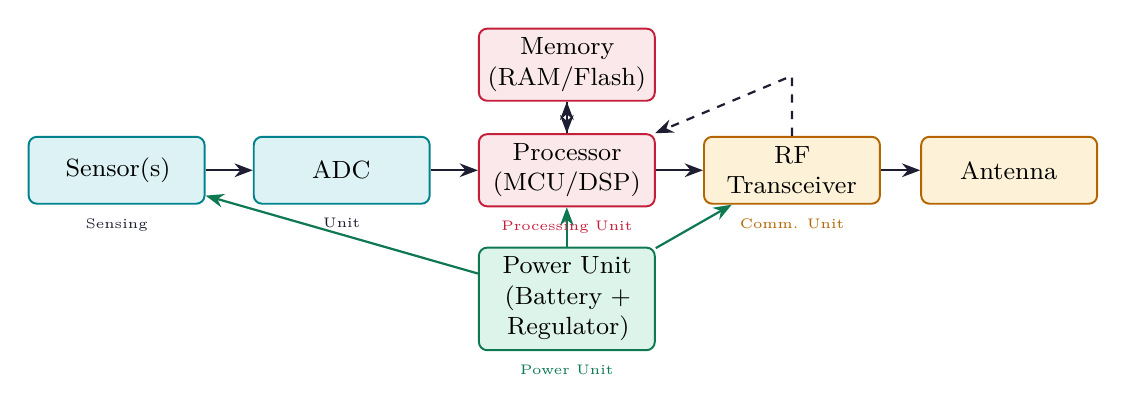
\begin{tikzpicture}[node distance=0.5cm and 0.8cm,
  sblock/.style={rectangle, draw=myteal, fill=hdrteal, text width=2.0cm,
    align=center, minimum height=0.85cm, font=\small,
    rounded corners=3pt, line width=0.7pt},
  rblock/.style={rectangle, draw=myred, fill=hdrred, text width=2.0cm,
    align=center, minimum height=0.85cm, font=\small,
    rounded corners=3pt, line width=0.7pt},
  ablock/.style={rectangle, draw=myamber, fill=hdramber, text width=2.0cm,
    align=center, minimum height=0.85cm, font=\small,
    rounded corners=3pt, line width=0.7pt},
  gblock/.style={rectangle, draw=mygreen, fill=hdrgreen, text width=2.0cm,
    align=center, minimum height=0.85cm, font=\small,
    rounded corners=3pt, line width=0.7pt}]

  % Row 1: Sensor + ADC
  \node[sblock] (sens)  {Sensor(s)};
  \node[sblock, right=0.6cm of sens] (adc) {ADC};

  % Processing unit
  \node[rblock, right=0.6cm of adc] (mcu) {Processor\\(MCU/DSP)};

  % Memory
  \node[rblock, above=0.4cm of mcu] (mem) {Memory\\(RAM/Flash)};

  % Communication
  \node[ablock, right=0.6cm of mcu] (trx) {RF\\Transceiver};
  \node[ablock, right=0.5cm of trx] (ant) {Antenna};

  % Power
  \node[gblock, below=0.5cm of mcu] (pwr) {Power Unit\\(Battery +\\Regulator)};

  % Arrows
  \draw[arrow] (sens) -- (adc);
  \draw[arrow] (adc) -- (mcu);
  \draw[arrow] (mcu) -- (trx);
  \draw[arrow] (trx) -- (ant);
  \draw[arrow, dashed] (trx) -- ++(0,1.2cm) -- (mcu);
  \draw[arrow] (mcu) -- (mem);
  \draw[arrow] (mem) -- (mcu);

  % Power supply arrows
  \draw[arrow, color=mygreen] (pwr) -- (sens);
  \draw[arrow, color=mygreen] (pwr) -- (mcu);
  \draw[arrow, color=mygreen] (pwr) -- (trx);

  % Labels
  \node[font=\tiny, color=mydark, below=0.05cm of sens] {Sensing};
  \node[font=\tiny, color=mydark, below=0.05cm of adc] {Unit};
  \node[font=\tiny, color=myred, below=0.05cm of mcu] {Processing Unit};
  \node[font=\tiny, color=myamber, below=0.05cm of trx] {Comm. Unit};
  \node[font=\tiny, color=mygreen, below=0.05cm of pwr] {Power Unit};
\end{tikzpicture}
\end{tcolorbox}

\subsection{Subsystems of a Sensor Node}

\subsubsection*{1. Sensing Unit}
Consists of one or more physical \textbf{sensors} and an \textbf{Analog-to-Digital Converter (ADC)}.
\begin{itemize}[leftmargin=*, itemsep=2pt]
  \item Sensor converts a physical parameter (temperature, light, pressure) into an analog electrical signal.
  \item ADC digitizes the analog signal for processing. Resolution: typically 8--12 bits. Sampling rate: application-dependent.
  \item Types of sensors used: resistive (NTC thermistor), capacitive (pressure), piezoelectric (vibration), MEMS accelerometers, optical (photodiode).
\end{itemize}

\subsubsection*{2. Processing Unit}
A \textbf{microcontroller (MCU)} that executes the embedded OS and application firmware.
\begin{itemize}[leftmargin=*, itemsep=2pt]
  \item Runs sensing schedule, data aggregation, routing protocol, and radio control.
  \item Includes on-chip \textbf{RAM} (2--10 KB) and \textbf{Flash} (32--256 KB).
  \item Examples: TI MSP430 (16-bit, 16 MHz, 165 $\mu$A active); ATmega128L (8-bit); ARM Cortex-M0.
\end{itemize}

\subsubsection*{3. Communication Unit}
A \textbf{wireless radio transceiver} operating in ISM band (typically 2.4 GHz or 868/915 MHz).
\begin{itemize}[leftmargin=*, itemsep=2pt]
  \item Implements IEEE 802.15.4 physical layer (O-QPSK modulation, 250 kbps).
  \item The radio is the most energy-hungry component: TX $\approx$ 17 mA, RX $\approx$ 20 mA; idle $\approx$ 1 mA; sleep $< 1$ $\mu$A.
  \item \textbf{Key design rule:} Duty-cycle the radio --- keep it in sleep mode as long as possible.
\end{itemize}

\subsubsection*{4. Power Unit}
Provides regulated voltage to all subsystems.
\begin{itemize}[leftmargin=*, itemsep=2pt]
  \item Primary source: AA or AAA alkaline batteries (1000--3000 mAh), lithium coin cells, or rechargeable LiPo.
  \item Energy harvesting can supplement: solar panels (thin-film), piezoelectric harvesters, thermoelectric generators.
  \item A low-dropout (LDO) regulator provides stable 3.3 V (or 1.8 V) rail.
\end{itemize}

% ===============================================================================
\section{Hardware Components and Design Constraints}
% ===============================================================================

\subsection{Key Hardware Components}

\par\noindent
{\renewcommand{\arraystretch}{1.5}%
\begin{tabularx}{\linewidth}{|B{3.0cm}|Y|Y|}
\hline
\textbf{Component} & \textbf{Function} & \textbf{Example / Spec} \\
\hline
\textbf{Sensor} & Convert physical quantity to electrical signal & NTC thermistor, MEMS accelerometer, CMOS image sensor \\
\hline
\textbf{ADC} & Digitize analog sensor output & 12-bit, 100 kSps, built into MCU \\
\hline
\textbf{Microcontroller} & Sensing, processing, routing decisions & TI MSP430, ATmega128L, ARM Cortex-M0 \\
\hline
\textbf{Memory (Flash)} & Store firmware, data logs & 64--256 KB on-chip; external SPI Flash \\
\hline
\textbf{Memory (RAM)} & Runtime data, routing tables, buffers & 2--10 KB on-chip \\
\hline
\textbf{RF Transceiver} & Wireless TX/RX & CC2420, CC2530 (IEEE 802.15.4); nRF24L01 \\
\hline
\textbf{Antenna} & Radiate/receive RF signal & Integrated PCB trace, chip antenna, wire monopole \\
\hline
\textbf{Battery} & Primary energy source & AA alkaline 2400 mAh; CR2032 coin 225 mAh \\
\hline
\textbf{LDO Regulator} & Stable voltage rail to all ICs & 3.3 V, 300 mA output \\
\hline
\textbf{Oscillator / RTC} & CPU clock and time-keeping & 32 kHz crystal for sleep; 8 MHz for active \\
\hline
\end{tabularx}}

\subsection{Design Constraints}

Design of a sensor node is governed by conflicting constraints that require careful trade-offs.

\begin{tcolorbox}[examplebox, title={\textbf{WSN Node Design Constraints}}]
\begin{enumerate}[leftmargin=*, itemsep=5pt]
  \item \textbf{Energy constraint:} Total energy $E = C \times V$. For a 2 AA cell pack (3 V, 2400 mAh) $= 7.2$ Wh. Every design decision must minimize current draw. \textbf{Radio sleep} is non-negotiable. Never keep the radio in RX idle --- this wastes as much power as transmitting.

  \item \textbf{Cost constraint:} Large-scale deployment requires node BOM cost $< $ Rs.~2000. This rules out GPS, high-quality ADCs, or large batteries. COTS low-cost transceivers (CC2520 $\approx$ Rs.~80) are used.

  \item \textbf{Size constraint:} Nodes must be small enough to embed in targets (soil probes, clothing, walls). PCB area typically $< 6 \times 6$ cm$^2$. This limits battery size and antenna length.

  \item \textbf{Memory constraint:} All code (OS + app + routing) must fit in 64--256 KB Flash. All runtime state in 4--10 KB RAM. Protocols must be algorithmically simple.

  \item \textbf{Communication range constraint:} IEEE 802.15.4 at 0 dBm TX gives $\sim$30 m indoor / $\sim$100 m outdoor range. Multi-hop routing extends coverage.

  \item \textbf{Reliability/robustness constraint:} Nodes must operate in extreme temperatures ($-20$°C to $+85$°C), humidity, and vibration. Industrial-grade MCUs and sealed enclosures are used.
\end{enumerate}
\end{tcolorbox}

\subsection{Energy Consumption Model}

The energy consumed by a node has four components:

\begin{tcolorbox}[formulabox, title={\textbf{Node Energy Model}}]
\[
E_{\text{node}} = E_{\text{sense}} + E_{\text{process}} + E_{\text{tx}} + E_{\text{rx}}
\]
\begin{itemize}[leftmargin=*, itemsep=4pt]
  \item $E_{\text{sense}} = I_{\text{sensor}} \times V \times t_{\text{sense}}$ \quad (sensor active time)
  \item $E_{\text{process}} = I_{\text{MCU\_active}} \times V \times t_{\text{process}}$
  \item $E_{\text{tx}} = (E_{\text{elec}} + \varepsilon_{\text{amp}} \cdot d^{\,n}) \times l$ \quad ($l$ = bits, $d$ = distance, $n=2$ or $4$)
  \item $E_{\text{rx}} = E_{\text{elec}} \times l$
\end{itemize}
\textbf{Key insight:} Communication energy $\gg$ computation energy. Reducing data volume (aggregation) and distance (clustering) drastically extends node lifetime.
\end{tcolorbox}

% ===============================================================================
\newpage
\section{Quick Revision --- Module 2}
% ===============================================================================

\begin{tcolorbox}[formulabox, title={\textbf{Key Formulas at a Glance}}]
\begin{itemize}[leftmargin=*, itemsep=4pt]
  \item Node energy budget: $E_{\text{node}} = E_{\text{sense}} + E_{\text{process}} + E_{\text{tx}} + E_{\text{rx}}$
  \item TX energy: $E_{tx}(l,d) = l \cdot E_{\text{elec}} + l \cdot \varepsilon_{\text{amp}} \cdot d^n$
  \item RX energy: $E_{rx}(l) = l \cdot E_{\text{elec}}$
  \item Node lifetime: $T = \dfrac{E_{\text{initial}}}{P_{\text{avg}}}$ \quad where $P_{\text{avg}}$ = average power draw
  \item Energy from battery: $E = Q \times V$ \quad (Q = capacity in Ah, V = voltage)
  \item Solar harvesting power: $P_{\text{solar}} = A \times \eta \times G$ \quad ($A$ = panel area, $\eta$ = efficiency, $G$ = irradiance)
\end{itemize}
\end{tcolorbox}

\begin{tcolorbox}[defbox, title={\textbf{One-Line Definitions}}]
\begin{itemize}[leftmargin=*, itemsep=3pt]
  \item \textbf{MANET:} Self-organizing mobile wireless network without fixed infrastructure; every node is both host and router.
  \item \textbf{Sensing unit:} Sensor + ADC subsystem that converts a physical quantity into a digital value.
  \item \textbf{Processing unit:} MCU + memory subsystem running the OS, application, and routing firmware.
  \item \textbf{Communication unit:} RF transceiver + antenna enabling wireless data exchange.
  \item \textbf{Power unit:} Battery + regulator providing stable power to all node subsystems.
  \item \textbf{MEMS:} Micro-Electro-Mechanical Systems --- miniaturized sensor fabrication technology enabling cheap, tiny transducers.
  \item \textbf{Energy harvesting:} Generating electricity from ambient sources (solar, vibration, thermal) to supplement or replace batteries.
  \item \textbf{Duty cycling:} Periodically turning off the radio (and MCU) to reduce average power; fundamental to WSN energy management.
\end{itemize}
\end{tcolorbox}

\begin{tcolorbox}[exambox, title={\textbf{Frequently Asked / Viva Questions --- Module 2}}]
\begin{enumerate}[leftmargin=*, itemsep=5pt]
  \item \Q{Compare MANET and WSN on at least five parameters.}
  MANET vs WSN: (1) Node capability --- MANET uses smartphones/laptops vs WSN uses resource-constrained motes; (2) Node count --- MANET few hundred vs WSN thousands; (3) Energy --- MANET moderate vs WSN critical; (4) Communication pattern --- MANET peer-to-peer vs WSN many-to-one to sink; (5) Addressing --- MANET IP-based vs WSN data-centric; (6) Data rate --- MANET Mbps vs WSN kbps.

  \item \Q{What are the enabling technologies that make WSNs feasible?}
  Six enabling technologies: (1) MEMS for miniaturized cheap sensors; (2) Low-power RF (IEEE 802.15.4) for energy-efficient wireless; (3) Low-power MCUs (MSP430) for $\mu$A-level sleep; (4) Energy harvesting (solar, piezo, thermal) for battery-less operation; (5) Lightweight embedded OSes (TinyOS, Contiki); (6) Cross-layer networking protocols (ZigBee, 6LoWPAN).

  \item \Q{Draw and explain the block diagram of a sensor node.}
  A sensor node has four subsystems: \textbf{Sensing unit} (sensors + ADC converts physical parameters to digital), \textbf{Processing unit} (MCU + RAM/Flash runs OS and algorithms), \textbf{Communication unit} (RF transceiver + antenna for wireless data), \textbf{Power unit} (battery + LDO regulator). All subsystems are co-designed for minimum energy.

  \item \Q{Why is the communication unit the most energy-hungry component of a sensor node?}
  The RF radio draws 17--20 mA in TX/RX vs 1--5 mA for the MCU and $<1$ mA for sensors. Even in idle listen mode the radio draws $\sim$1 mA --- equivalent to thousands of MCU sleep cycles. This makes radio duty-cycling (aggressive sleep scheduling) the primary energy optimization technique.

  \item \Q{What is MEMS and how does it enable WSN?}
  MEMS (Micro-Electro-Mechanical Systems) uses semiconductor fabrication techniques to build mechanical structures (membranes, cantilevers) alongside electronics on a single chip. This creates cheap ($<$ Rs.~50), tiny, low-power sensors for temperature, pressure, acceleration, and gas detection --- prerequisites for mass-deployable WSN nodes.

  \item \Q{List and briefly explain the six design constraints of a sensor node.}
  (1) \textbf{Energy} --- limited non-rechargeable battery; (2) \textbf{Cost} --- mass deployment, Rs.~100--2000 per node; (3) \textbf{Size} --- PCB must be compact ($< 6 \times 6$ cm); (4) \textbf{Memory} --- only KB-level RAM/Flash; (5) \textbf{Communication range} --- 10--100 m; (6) \textbf{Reliability} --- must work in harsh environments.

  \item \Q{What is energy harvesting? Give three examples used in WSN.}
  Energy harvesting captures ambient energy and converts it into electrical energy to supplement or replace batteries. Examples: (1) \textbf{Solar:} Photovoltaic cells convert light to electricity (10--100 mW/cm$^2$ outdoor); (2) \textbf{Piezoelectric:} Mechanical vibrations deform piezo material generating voltage; (3) \textbf{Thermoelectric:} Seebeck effect converts temperature gradient across a thermoelectric module into voltage.

  \item \Q{What is the hidden terminal problem in WSNs?}
  Nodes A and C are both in range of B but not of each other. When A and C simultaneously transmit to B, their signals collide at B. Neither A nor C detects the collision (they cannot hear each other). This is the hidden terminal problem, solved using RTS/CTS handshaking or CSMA with virtual carrier sensing.

  \item \Q{What is duty cycling and why is it critical in WSN?}
  Duty cycling = fraction of time the radio (or MCU) is ON. If a node transmits 1 ms every 1 s, duty cycle = 0.1\%. If idle-listen current = 20 mA and duty cycle = 1\%, average current $\approx 0.2$ mA --- extending a 2000 mAh battery from $\sim$4 days (always-on) to $\sim$400 days.

  \item \Q{How does a sensor convert a physical quantity to digital data?}
  The physical quantity (e.g., temperature) changes the sensor's electrical property (e.g., NTC thermistor resistance). This is connected in a voltage divider; the analog voltage is fed to an \textbf{ADC} (Analog-to-Digital Converter). The ADC samples the voltage and quantizes it to $n$-bit digital code (e.g., 12-bit = 4096 levels) for the MCU.

  \item \Q{Name two lightweight embedded OSes used in WSN and one property each.}
  (1) \textbf{TinyOS:} Event-driven, component-based OS developed at UC Berkeley for motes; fits in $<$ 4 KB RAM. (2) \textbf{Contiki:} Protothreads-based OS supporting IPv6/6LoWPAN; enables internet connectivity for sensor nodes.

  \item \Q{What is the significance of the radio transceiver's idle-listen state?}
  In idle-listen, the radio is powered ON and listening but no data is being received. Current draw is similar to receive mode ($\sim$20 mA). A protocol that leaves the radio always-on in idle-listen wastes enormous energy even with no traffic. This motivates sleep-wake scheduling MAC protocols (S-MAC, TDMA) that turn off the radio between duty cycles.
\end{enumerate}
\end{tcolorbox}

\begin{tcolorbox}[tikzbox, title={\textbf{Summary: MANET vs WSN at a Glance}}]
\par\noindent
{\renewcommand{\arraystretch}{1.4}%
\begin{tabularx}{\linewidth}{|B{2.8cm}|Y|Y|}
\hline
\textbf{Attribute} & \textbf{MANET} & \textbf{WSN} \\
\hline
Node capability & High & Very low \\
\hline
Energy priority & Moderate & Critical \\
\hline
Traffic pattern & Peer-to-peer & Many-to-one \\
\hline
Addressing & IP-based & Data-centric \\
\hline
Deployment & Planned & Random \\
\hline
Node failures & Exceptional & Expected \\
\hline
\end{tabularx}}
\end{tcolorbox}


% -- Module 3 -----------------------------------------------------------------
\modulestart{3}{MAC Protocols for WSN}

\section{MAC Protocols for WSN}
% ===============================================================================

\begin{tcolorbox}[defbox, title={\textbf{MAC Protocol --- Definition}}]
A \textbf{Medium Access Control (MAC) protocol} governs how sensor nodes share the common wireless channel. In WSN, the MAC layer has an additional critical responsibility: \textbf{energy management} --- scheduling the radio's sleep/wake cycle to minimize idle listening, overhearing, and collision-related retransmissions.
\end{tcolorbox}

\subsection{Major Energy Waste Sources at MAC Layer}
\begin{itemize}[leftmargin=*, itemsep=3pt]
  \item \textbf{Idle listening:} Radio is ON but no packet arrives --- most wasteful (equal to RX energy).
  \item \textbf{Overhearing:} A node receives a packet destined for another node.
  \item \textbf{Collision:} Two nodes transmit simultaneously; packets are corrupt and must be retransmitted.
  \item \textbf{Control packet overhead:} RTS/CTS/ACK consume energy without carrying data.
  \item \textbf{Overmitting:} Transmitting to a node not yet ready to receive.
\end{itemize}

% ===============================================================================
\section{Classification of MAC Protocols}
% ===============================================================================

WSN MAC protocols are broadly classified as:

\par\noindent
{\renewcommand{\arraystretch}{1.5}%
\begin{tabularx}{\linewidth}{|B{3.0cm}|Y|Y|Y|}
\hline
\textbf{Category} & \textbf{Mechanism} & \textbf{Advantages} & \textbf{Disadvantages} \\
\hline
\textbf{Contention-based (CSMA family)} & Nodes contend for channel; random back-off on collision & Simple, no coordination needed, handles variable load & Collisions, idle listening, scalability issues \\
\hline
\textbf{Schedule-based (TDMA family)} & Nodes assigned fixed time slots; radio OFF in other slots & Collision-free, predictable energy, no idle listening & Requires synchronization, poor adaptability \\
\hline
\textbf{Hybrid} & Combines TDMA + CSMA dynamically & Balanced energy and adaptability & Complex design \\
\hline
\end{tabularx}}

% ===============================================================================
\section{S-MAC Protocol (Sensor-MAC)}
% ===============================================================================

\begin{tcolorbox}[defbox, title={\textbf{S-MAC --- Definition}}]
\textbf{S-MAC (Sensor-MAC)} is a contention-based MAC protocol for WSN that introduces \textbf{periodic sleep--wake schedules} for all nodes in a neighborhood. Nodes synchronize their schedules, go to sleep during idle periods, and wake up to exchange data only during active periods, dramatically reducing idle-listen energy.
\end{tcolorbox}

\subsection{S-MAC Working Principle}

\begin{enumerate}[leftmargin=*, itemsep=4pt]
  \item \textbf{Listen--Sleep schedule:} Time is divided into frames. Each frame has a \textbf{LISTEN} period and a \textbf{SLEEP} period. All nodes in a cluster share the same schedule.
  \item \textbf{Schedule exchange (SYNC):} On startup, a node listens for SYNC packets. If it hears a neighbor's schedule, it adopts it. Otherwise it creates its own and broadcasts a SYNC packet.
  \item \textbf{Data exchange:} Data is sent only during the LISTEN period using CSMA with RTS/CTS.
  \item \textbf{In-band signaling:} A NAV (Network Allocation Vector) field in RTS/CTS tells neighboring nodes how long to stay asleep (virtual carrier sensing).
  \item \textbf{Message passing:} For long messages, S-MAC uses message passing where a node stays awake for consecutive frames to receive the entire message --- reduces latency.
\end{enumerate}

\subsection{S-MAC Frame Structure}

\begin{tcolorbox}[tikzbox, title={S-MAC Sleep--Wake Schedule}]
\centering
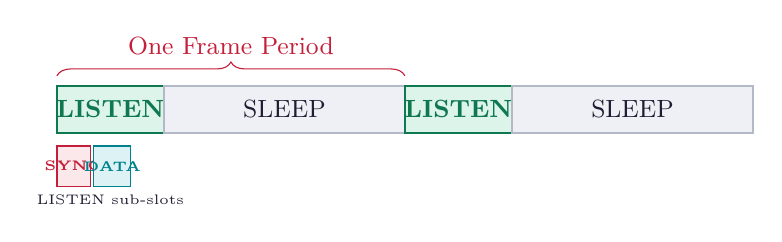
\begin{tikzpicture}[scale=0.85]
  % Frame 1
  \draw[fill=hdrgreen, draw=mygreen, line width=0.7pt] (0,0) rectangle (1.6,0.7);
  \node[font=\small\bfseries, color=mygreen] at (0.8,0.35) {LISTEN};
  \draw[fill=hdrgray, draw=mgframe, line width=0.7pt] (1.6,0) rectangle (5.2,0.7);
  \node[font=\small, color=mydark] at (3.4,0.35) {SLEEP};
  % Frame 2
  \draw[fill=hdrgreen, draw=mygreen, line width=0.7pt] (5.2,0) rectangle (6.8,0.7);
  \node[font=\small\bfseries, color=mygreen] at (6.0,0.35) {LISTEN};
  \draw[fill=hdrgray, draw=mgframe, line width=0.7pt] (6.8,0) rectangle (10.4,0.7);
  \node[font=\small, color=mydark] at (8.6,0.35) {SLEEP};

  % Brace
  \draw[decorate, decoration={brace, amplitude=5pt}, color=myred]
    (0,0.85) -- (5.2,0.85) node[midway, above=4pt, font=\small, color=myred] {One Frame Period};

  % Labels under LISTEN
  \draw[fill=hdrred, draw=myred, line width=0.5pt] (0,-0.8) rectangle (0.5,-0.2);
  \node[font=\tiny\bfseries, color=myred] at (0.25,-0.5) {SYNC};
  \draw[fill=hdrteal, draw=myteal, line width=0.5pt] (0.55,-0.8) rectangle (1.1,-0.2);
  \node[font=\tiny\bfseries, color=myteal] at (0.825,-0.5) {DATA};
  \node[font=\tiny, color=mydark] at (0.8,-1.0) {LISTEN sub-slots};
\end{tikzpicture}
\end{tcolorbox}

\subsection{S-MAC: Advantages and Disadvantages}

\par\noindent
{\renewcommand{\arraystretch}{1.5}%
\begin{tabularx}{\linewidth}{|Y|Y|}
\hline
\textbf{Advantages} & \textbf{Disadvantages} \\
\hline
Reduces idle listening significantly & Fixed duty cycle may waste energy at low traffic \\
\hline
Simple schedule coordination (SYNC packets) & Increased latency due to sleep periods \\
\hline
Collision avoidance via virtual carrier sense (NAV) & Border nodes may follow two schedules, reducing sleep time \\
\hline
Works well in dense, static networks & Not adaptive to varying traffic loads \\
\hline
\end{tabularx}}

% ===============================================================================
\section{B-MAC Protocol (Berkeley-MAC)}
% ===============================================================================

\begin{tcolorbox}[defbox, title={\textbf{B-MAC --- Definition}}]
\textbf{B-MAC (Berkeley-MAC)} is a contention-based MAC protocol that uses \textbf{Low-Power Listening (LPL)} (also called \textbf{preamble sampling}) to reduce idle-listen energy. A node wakes up briefly at intervals to check for channel activity (preamble) and only stays awake if it detects a transmission directed to it.
\end{tcolorbox}

\subsection{B-MAC Low-Power Listening (LPL) Mechanism}

\begin{enumerate}[leftmargin=*, itemsep=4pt]
  \item \textbf{Receiver side:} Each node wakes up periodically (every check interval $T_c$) for a short duration ($\sim$1 ms), samples the channel using Clear Channel Assessment (CCA).
  \begin{itemize}
    \item If channel is idle: back to sleep.
    \item If channel is busy: stay awake and receive the full packet.
  \end{itemize}
  \item \textbf{Sender side:} Before data, the sender transmits a \textbf{long preamble} of duration $\geq T_c$ (the check interval). This ensures the receiver wakes up at least once and detects the preamble.
  \item After detecting the preamble, the receiver stays awake and receives the data packet.
\end{enumerate}

\begin{tcolorbox}[tikzbox, title={B-MAC Low-Power Listening --- Timing}]
\centering
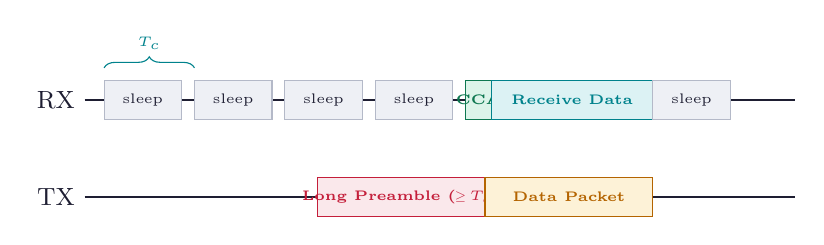
\begin{tikzpicture}[scale=0.82]
  % Receiver timeline
  \draw[thick, color=mydark] (0,1.5) -- (11,1.5);
  \node[left, font=\small, color=mydark] at (0,1.5) {RX};
  % Sleep pulses
  \foreach \x in {0.3, 1.7, 3.1, 4.5} {
    \draw[fill=hdrgray, draw=mgframe] (\x,1.2) rectangle (\x+1.2,1.8);
    \node[font=\tiny, color=mydark] at (\x+0.6,1.5) {sleep};
  }
  % Wake up sample
  \draw[fill=hdrgreen, draw=mygreen] (5.9,1.2) rectangle (6.3,1.8);
  \node[font=\tiny\bfseries, color=mygreen] at (6.1,1.5) {CCA};
  % Stay awake + receive
  \draw[fill=hdrteal, draw=myteal] (6.3,1.2) rectangle (8.8,1.8);
  \node[font=\tiny\bfseries, color=myteal] at (7.55,1.5) {Receive Data};
  % Back to sleep
  \draw[fill=hdrgray, draw=mgframe] (8.8,1.2) rectangle (10.0,1.8);
  \node[font=\tiny, color=mydark] at (9.4,1.5) {sleep};

  % Sender timeline
  \draw[thick, color=mydark] (0,0) -- (11,0);
  \node[left, font=\small, color=mydark] at (0,0) {TX};
  \draw[fill=hdrred, draw=myred] (3.6,-0.3) rectangle (6.2,0.3);
  \node[font=\tiny\bfseries, color=myred] at (4.9,0.0) {Long Preamble ($\geq T_c$)};
  \draw[fill=hdramber, draw=myamber] (6.2,-0.3) rectangle (8.8,0.3);
  \node[font=\tiny\bfseries, color=myamber] at (7.5,0.0) {Data Packet};

  % Brace for check interval
  \draw[decorate, decoration={brace, amplitude=4pt}, color=myteal]
    (0.3,2.0) -- (1.7,2.0) node[midway, above=3pt, font=\tiny, color=myteal] {$T_c$};
\end{tikzpicture}
\end{tcolorbox}

\subsection{B-MAC vs S-MAC}

\par\noindent
{\renewcommand{\arraystretch}{1.5}%
\begin{tabularx}{\linewidth}{|B{3.0cm}|Y|Y|}
\hline
\textbf{Parameter} & \textbf{S-MAC} & \textbf{B-MAC} \\
\hline
\textbf{Approach} & Synchronized sleep schedules & Asynchronous preamble sampling \\
\hline
\textbf{Synchronization} & Required (SYNC packets) & Not required \\
\hline
\textbf{Latency} & Higher (must wait for LISTEN period) & Lower (no schedule dependency) \\
\hline
\textbf{Preamble overhead} & Short & Long (= check interval) \\
\hline
\textbf{Adaptability} & Fixed duty cycle & Check interval tunable per traffic load \\
\hline
\textbf{Complexity} & Moderate & Low \\
\hline
\end{tabularx}}

% ===============================================================================
\section{IEEE 802.15.4 Standard}
% ===============================================================================

\begin{tcolorbox}[defbox, title={\textbf{IEEE 802.15.4 --- Definition}}]
\textbf{IEEE 802.15.4} is the wireless standard defining the \textbf{Physical (PHY)} and \textbf{MAC} layers for Low-Rate Wireless Personal Area Networks (LR-WPANs). It is the foundation protocol used by ZigBee, 6LoWPAN, Thread, and WirelessHART. It targets low data rate, low power, and low cost sensor/actuator applications.
\end{tcolorbox}

\subsection{Key Specifications of IEEE 802.15.4}

\par\noindent
{\renewcommand{\arraystretch}{1.5}%
\begin{tabularx}{\linewidth}{|B{3.4cm}|Y|}
\hline
\textbf{Parameter} & \textbf{Value / Description} \\
\hline
\textbf{Frequency band} & 2.4 GHz (global), 915 MHz (Americas), 868 MHz (Europe) \\
\hline
\textbf{Data rate} & 250 kbps (2.4 GHz); 40 kbps (915 MHz); 20 kbps (868 MHz) \\
\hline
\textbf{Range} & 10--100 m (LOS); 10--30 m indoor \\
\hline
\textbf{TX power} & $-3$ dBm to $+3$ dBm (1--2 mW) \\
\hline
\textbf{Modulation} & O-QPSK (2.4 GHz), BPSK (868/915 MHz) \\
\hline
\textbf{Channels} & 16 channels at 2.4 GHz (Ch. 11--26, 5 MHz spacing) \\
\hline
\textbf{Addressing} & 16-bit short or 64-bit extended IEEE address \\
\hline
\textbf{Network topology} & Star or peer-to-peer (mesh) \\
\hline
\textbf{Security} & AES-128 encryption optional \\
\hline
\end{tabularx}}

\subsection{Device Types in IEEE 802.15.4}
\begin{itemize}[leftmargin=*, itemsep=3pt]
  \item \textbf{Full Function Device (FFD):} Can act as coordinator, router, or end device. Supports all MAC functions.
  \item \textbf{Reduced Function Device (RFD):} Simplified device; can only communicate with a coordinator. Cannot relay packets. Lower cost, lower power.
  \item \textbf{PAN Coordinator:} The master FFD of the network; manages the PAN (Personal Area Network), assigns addresses, and generates beacon frames.
\end{itemize}

\subsection{Superframe Structure}

IEEE 802.15.4 optionally uses a \textbf{beacon-enabled superframe} structure for scheduled access:

\begin{itemize}[leftmargin=*, itemsep=3pt]
  \item \textbf{Beacon:} Sent by PAN coordinator to synchronize all devices.
  \item \textbf{CAP (Contention Access Period):} CSMA-CA based contention slots for general data.
  \item \textbf{CFP (Contention-Free Period):} Guaranteed Time Slots (GTS) assigned to specific devices --- collision-free, low latency.
  \item \textbf{Inactive period:} All nodes sleep; radio off.
\end{itemize}

% ===============================================================================
\section{ZigBee}
% ===============================================================================

\begin{tcolorbox}[defbox, title={\textbf{ZigBee --- Definition}}]
\textbf{ZigBee} is a high-level wireless communication protocol stack built on top of IEEE 802.15.4 (PHY + MAC layers). It adds the \textbf{Network Layer (NWK)} and \textbf{Application Layer (APL)} to enable mesh networking, self-healing, multi-hop routing, and device/service discovery for IoT and WSN applications.
\end{tcolorbox}

\subsection{ZigBee Protocol Stack}

\begin{tcolorbox}[tikzbox, title={ZigBee Protocol Stack Layers}]
\centering
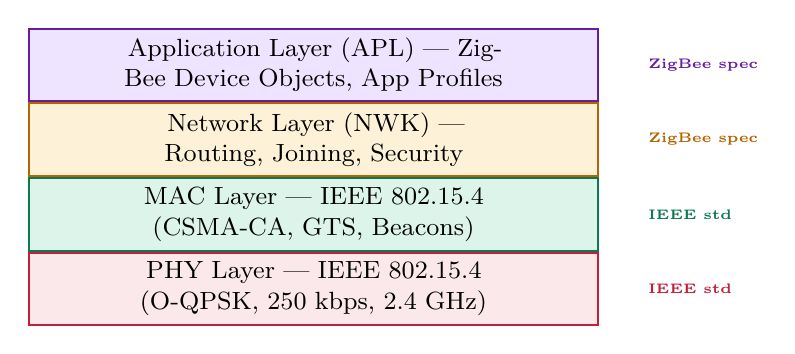
\begin{tikzpicture}[node distance=0cm,
  layer/.style={rectangle, draw=myteal, fill=hdrteal, text width=7cm,
    align=center, minimum height=0.65cm, font=\small, line width=0.7pt}]
  \node[layer, fill=hdrpurple, draw=mypurple] (apl) {Application Layer (APL) --- ZigBee Device Objects, App Profiles};
  \node[layer, fill=hdramber, draw=myamber, below=0cm of apl] (nwk) {Network Layer (NWK) --- Routing, Joining, Security};
  \node[layer, fill=hdrgreen, draw=mygreen, below=0cm of nwk] (mac) {MAC Layer --- IEEE 802.15.4 (CSMA-CA, GTS, Beacons)};
  \node[layer, fill=hdrred, draw=myred, below=0cm of mac] (phy) {PHY Layer --- IEEE 802.15.4 (O-QPSK, 250 kbps, 2.4 GHz)};

  \node[right=0.5cm of apl, font=\tiny, color=mypurple, align=left] {\textbf{ZigBee spec}};
  \node[right=0.5cm of nwk, font=\tiny, color=myamber, align=left] {\textbf{ZigBee spec}};
  \node[right=0.5cm of mac, font=\tiny, color=mygreen, align=left] {\textbf{IEEE std}};
  \node[right=0.5cm of phy, font=\tiny, color=myred, align=left] {\textbf{IEEE std}};
\end{tikzpicture}
\end{tcolorbox}

\subsection{ZigBee Device Types}
\begin{itemize}[leftmargin=*, itemsep=3pt]
  \item \textbf{ZigBee Coordinator (ZC):} One per network; initiates network formation, stores network map, and bridges to other networks.
  \item \textbf{ZigBee Router (ZR):} Participates in routing; relays data for other nodes; always-on (not battery-optimized).
  \item \textbf{ZigBee End Device (ZED):} Leaf node; communicates only with its parent (coordinator or router); can sleep aggressively; lowest power.
\end{itemize}

\subsection{ZigBee Network Topologies}
\begin{itemize}[leftmargin=*, itemsep=3pt]
  \item \textbf{Star:} All devices communicate directly to the coordinator. Simple, limited range.
  \item \textbf{Tree (Cluster tree):} Hierarchical network; data flows up the tree toward the coordinator. Scalable.
  \item \textbf{Mesh:} Any router can communicate with any other router. Self-healing; most robust; supports AODV-based routing.
\end{itemize}

% ===============================================================================
\section{Routing Protocols for WSN}
% ===============================================================================

Routing in WSN must be energy-aware, since the network lifetime depends on balancing energy consumption across nodes.

\subsection{Flooding and Gossiping}

\begin{itemize}[leftmargin=*, itemsep=3pt]
  \item \textbf{Flooding:} A node broadcasts a packet to all neighbors; each receiving node rebroadcasts to its neighbors, and so on. Simple but causes \textbf{implosion} (same data arrives at a node multiple times), \textbf{overlap} (nearby nodes sense same region and send duplicate data), and \textbf{resource blindness} (does not consider node energy).
  \item \textbf{Gossiping:} Instead of broadcasting, a node randomly selects one neighbor and forwards the packet. Reduces implosion but creates random latency.
\end{itemize}

\subsection{SPIN (Sensor Protocols for Information via Negotiation)}

\begin{tcolorbox}[defbox, title={\textbf{SPIN --- Definition}}]
\textbf{SPIN} is a data-centric routing protocol that uses \textbf{metadata negotiation} to eliminate redundant transmissions. Nodes advertise data descriptors (meta-data) before sending actual data, and only nodes that do not have the data request it.
\end{tcolorbox}

SPIN uses three message types:
\begin{itemize}[leftmargin=*, itemsep=2pt]
  \item \textbf{ADV:} Advertisement --- ``I have new data with this descriptor''.
  \item \textbf{REQ:} Request --- ``I want that data''.
  \item \textbf{DATA:} Actual data payload.
\end{itemize}

\subsection{Directed Diffusion}

\begin{tcolorbox}[defbox, title={\textbf{Directed Diffusion --- Definition}}]
\textbf{Directed Diffusion} is a data-centric, interest-driven routing protocol where the sink \textbf{floods interests} (queries) into the network. Sensor nodes that have matching data respond by sending data along the gradient (path) that was set up by the interest. Reinforcement is used to select the best path.
\end{tcolorbox}

Three phases:
\begin{enumerate}[leftmargin=*, itemsep=3pt]
  \item \textbf{Interest propagation:} Sink broadcasts interest (query) with parameters (attribute=value pairs, duration, frequency).
  \item \textbf{Gradient setup:} Each intermediate node records the direction of the interest source and sets up a gradient toward the sink.
  \item \textbf{Data delivery + Path reinforcement:} Data flows back along gradients. The sink reinforces the best-quality path by increasing data rate on that path; other gradients are suppressed.
\end{enumerate}

\subsection{LEACH Protocol (Low-Energy Adaptive Clustering Hierarchy)}

\begin{tcolorbox}[defbox, title={\textbf{LEACH --- Definition}}]
\textbf{LEACH} is a hierarchical, cluster-based routing protocol for WSN that distributes energy load by rotating the \textbf{Cluster Head (CH)} role among all nodes in rounds. Each CH aggregates data from its cluster members and forwards compressed data to the base station via single-hop.
\end{tcolorbox}

\subsubsection*{LEACH Operation: Two Phases per Round}

\textbf{Phase 1 --- Setup Phase:}
\begin{itemize}[leftmargin=*, itemsep=2pt]
  \item Each node decides to become a CH with probability $p$:
\end{itemize}

\begin{tcolorbox}[formulabox, title={\textbf{LEACH --- Cluster Head Probability}}]
\[
P(n) = \begin{cases}
\dfrac{p}{1 - p \cdot (r \bmod \frac{1}{p})} & \text{if } n \notin G \\
0 & \text{if } n \in G
\end{cases}
\]
where $p$ = desired fraction of CHs (typically 0.05 = 5\%), $r$ = current round number, $G$ = set of nodes that were CHs in the last $1/p$ rounds.

\textbf{Optimal CH fraction:} $p_{\text{opt}} = \sqrt{\dfrac{A}{2\pi}} \cdot \dfrac{1}{d_{BS}} \cdot \sqrt{\dfrac{\varepsilon_{\text{fs}}}{\varepsilon_{\text{mp}}}}$

where $A$ = field area, $d_{BS}$ = distance to base station.
\end{tcolorbox}

\begin{itemize}[leftmargin=*, itemsep=2pt]
  \item Nodes that become CHs broadcast an advertisement. Non-CH nodes join the nearest CH (based on RSSI).
  \item CH creates a TDMA schedule for its cluster members.
\end{itemize}

\textbf{Phase 2 --- Steady-State Phase:}
\begin{itemize}[leftmargin=*, itemsep=2pt]
  \item Cluster members transmit data in their assigned TDMA slot; radio is OFF in other slots.
  \item CH aggregates received data and transmits compressed aggregate to base station using long-range radio.
  \item After a fixed number of frames, a new setup phase begins with new CH selection.
\end{itemize}

\begin{tcolorbox}[tikzbox, title={LEACH Cluster Formation Diagram}]
\centering
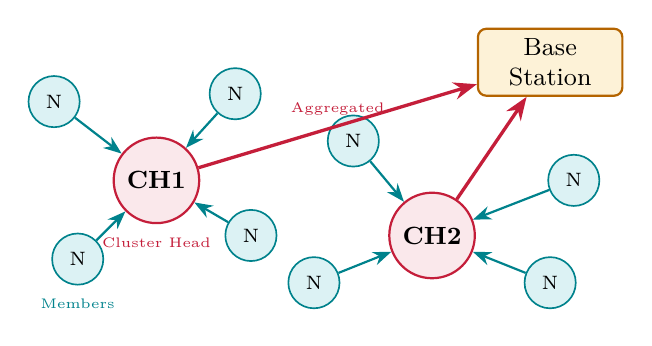
\begin{tikzpicture}[node distance=0.4cm,
  chnode/.style={circle, draw=myred, fill=hdrred, minimum size=1.0cm, font=\small\bfseries, line width=0.8pt},
  mnode/.style={circle, draw=myteal, fill=hdrteal, minimum size=0.65cm, font=\scriptsize, line width=0.6pt},
  bsnode/.style={rectangle, draw=myamber, fill=hdramber, text width=1.6cm, align=center, minimum height=0.85cm, font=\small, rounded corners=3pt, line width=0.8pt}]

  % Base Station
  \node[bsnode] (bs) at (6.5,3.0) {Base Station};

  % Cluster 1 CH
  \node[chnode] (ch1) at (1.5, 1.5) {CH1};
  % Cluster 1 members
  \node[mnode] (m11) at (0.2, 2.5) {N};
  \node[mnode] (m12) at (0.5, 0.5) {N};
  \node[mnode] (m13) at (2.5, 2.6) {N};
  \node[mnode] (m14) at (2.7, 0.8) {N};

  % Cluster 2 CH
  \node[chnode] (ch2) at (5.0, 0.8) {CH2};
  % Cluster 2 members
  \node[mnode] (m21) at (3.5, 0.2) {N};
  \node[mnode] (m22) at (4.0, 2.0) {N};
  \node[mnode] (m23) at (6.5, 0.2) {N};
  \node[mnode] (m24) at (6.8, 1.5) {N};

  % Member to CH arrows
  \draw[arrow, color=myteal] (m11) -- (ch1);
  \draw[arrow, color=myteal] (m12) -- (ch1);
  \draw[arrow, color=myteal] (m13) -- (ch1);
  \draw[arrow, color=myteal] (m14) -- (ch1);
  \draw[arrow, color=myteal] (m21) -- (ch2);
  \draw[arrow, color=myteal] (m22) -- (ch2);
  \draw[arrow, color=myteal] (m23) -- (ch2);
  \draw[arrow, color=myteal] (m24) -- (ch2);

  % CH to BS arrows
  \draw[redarrow, line width=1.2pt] (ch1) -- (bs) node[midway, above, font=\tiny, color=myred] {Aggregated};
  \draw[redarrow, line width=1.2pt] (ch2) -- (bs);

  % Labels
  \node[font=\tiny, color=myred, below=0.05cm of ch1] {Cluster Head};
  \node[font=\tiny, color=myteal, below=0.05cm of m12] {Members};
\end{tikzpicture}
\end{tcolorbox}

\subsection{TEEN and APTEEN Protocols}

For applications with time-critical events, standard proactive clustering like LEACH is inefficient because it transmits data periodically even when there is no change in the sensed environment. Hierarchical routing has reactive and hybrid extensions:

\begin{tcolorbox}[defbox, title={\textbf{TEEN (Threshold sensitive Energy Efficient sensor Network) --- Definition}}]
\textbf{TEEN} is a \textbf{reactive} hierarchical routing protocol designed for time-critical applications. Motes sense their environment continuously, but only transmit data to their cluster heads if the sensed value crosses a \textbf{Hard Threshold ($H_T$)} (to trigger on events of interest) and changes by an amount equal to or greater than a \textbf{Soft Threshold ($S_T$)} (to reduce transmission of small, insignificant fluctuations).
\end{tcolorbox}

\textbf{TEEN Threshold Conditions for Transmission:}
Let $V_{\text{sensed}}$ be the current sensed value, and $V_{\text{last\_tx}}$ be the value of the last transmitted data. A node transmits if and only if:
\[
(V_{\text{sensed}} > H_T) \quad \land \quad (|V_{\text{sensed}} - V_{\text{last\_tx}}| \geq S_T)
\]
\begin{itemize}[leftmargin=*, itemsep=3pt]
  \item \textbf{Hard Threshold ($H_T$):} The absolute value above which a sensor node must turn on its transmitter and report (e.g., Temperature $> 60^\circ$C).
  \item \textbf{Soft Threshold ($S_T$):} A small change in the value of the sensed attribute that triggers the node to transmit again (e.g., change of $\ge 2^\circ$C).
\end{itemize}

\begin{tcolorbox}[defbox, title={\textbf{APTEEN (Adaptive Periodic Threshold sensitive Energy Efficient) --- Definition}}]
\textbf{APTEEN} is a \textbf{hybrid} protocol that extends TEEN to support both periodic (proactive) data collection and event-driven (reactive) transmissions. It allows the user to specify a \textbf{Count Time ($T_C$)}: if a node does not send data for a duration equal to $T_C$, it is forced to transmit its current reading, ensuring the user receives regular heartbeats.
\end{tcolorbox}

\textbf{Comparison: LEACH vs. TEEN vs. APTEEN}

\par\noindent
{\renewcommand{\arraystretch}{1.4}%
\begin{tabularx}{\linewidth}{|B{2.8cm}|Y|Y|Y|}
\hline
\textbf{Parameter} & \textbf{LEACH} & \textbf{TEEN} & \textbf{APTEEN} \\
\hline
\textbf{Network Type} & Proactive (periodic) & Reactive (event-driven) & Hybrid (periodic + event) \\
\hline
\textbf{Data transmission} & Continuous at time slots & Only when thresholds met & Periodic + threshold triggers \\
\hline
\textbf{Energy efficiency} & Moderate & Very High & High \\
\hline
\textbf{Delay} & Higher (scheduled) & Minimal (immediate TX) & Minimal for events \\
\hline
\textbf{Best suited for} & Constant monitoring & Disaster/fire detection & Dynamic query systems \\
\hline
\end{tabularx}}

\subsection{Location-Based (Geographic) Routing Protocols}

Geographic routing protocols use geographic coordinates (localization or GPS) to route data, eliminating the need to maintain routing tables or flood interests.

\begin{tcolorbox}[defbox, title={\textbf{GEAR (Geographical and Energy-Aware Routing) --- Definition}}]
\textbf{GEAR} is a location-based routing protocol that routes queries to a target region using geographic coordinates and remaining energy levels of neighbors. It replaces interest flooding (in Directed Diffusion) with localized geographic forwarding to the target region, saving significant energy.
\end{tcolorbox}

\textbf{GEAR Forwarding Strategy:}
\begin{itemize}[leftmargin=*, itemsep=2pt]
  \item A node forwards packets to the neighbor closest to the target region that has high remaining energy.
  \item If a node encounters a ``hole'' (no neighbor is closer to the target than itself), it routes using a \textbf{learned cost} based on neighbor energy and distance.
\end{itemize}

\begin{tcolorbox}[defbox, title={\textbf{GAF (Geographic Adaptive Fidelity) --- Definition}}]
\textbf{GAF} is an energy-conserving location-based routing protocol that divides the network area into a \textbf{virtual grid}. Since all nodes within a grid cell can route packets to adjacent cells equally, GAF keeps only \textbf{one node active} in each cell while putting all other nodes in a low-power sleep state, maximizing network lifetime.
\end{tcolorbox}

\textbf{GAF Grid Size Constraint:}
To ensure any node in a grid cell $(x, y)$ can communicate with any node in adjacent cells (like $(x+1, y)$), the grid cell size $r$ must satisfy:
\[
r \leq \frac{R}{\sqrt{5}}
\]
where $R$ is the wireless transmission range of the nodes.

% ===============================================================================
\newpage
\section{Quick Revision --- Module 3}
% ===============================================================================

\begin{tcolorbox}[formulabox, title={\textbf{Key Formulas at a Glance}}]
\begin{itemize}[leftmargin=*, itemsep=4pt]
  \item LEACH CH probability: $P(n) = \dfrac{p}{1 - p \cdot (r \bmod \frac{1}{p})}$ for non-recent CH nodes; 0 otherwise
  \item Optimal CH fraction: $p_{\text{opt}} \propto \dfrac{1}{d_{BS}} \cdot \sqrt{\dfrac{\varepsilon_{\text{fs}}}{\varepsilon_{\text{mp}}}}$
  \item TEEN transmission condition: $(V_{\text{sensed}} > H_T) \land (|V_{\text{sensed}} - V_{\text{last\_tx}}| \geq S_T)$
  \item GAF grid cell size constraint: $r \leq \dfrac{R}{\sqrt{5}}$ \quad ($R$ = transmission range)
  \item B-MAC preamble length: $T_{\text{preamble}} \geq T_{\text{check}}$ (check interval of receiver)
\end{itemize}
\end{tcolorbox}

\begin{tcolorbox}[defbox, title={\textbf{One-Line Definitions}}]
\begin{itemize}[leftmargin=*, itemsep=3pt]
  \item \textbf{S-MAC:} Synchronized sleep-wake MAC; nodes share a schedule and sleep during idle periods.
  \item \textbf{B-MAC:} Preamble sampling MAC; receiver wakes briefly to check for long preamble before receiving.
  \item \textbf{IEEE 802.15.4:} PHY+MAC standard for LR-WPAN; 250 kbps at 2.4 GHz; foundation of ZigBee.
  \item \textbf{ZigBee:} Network+application layer stack on IEEE 802.15.4; mesh routing, self-healing, IoT standard.
  \item \textbf{SPIN:} Metadata negotiation protocol --- nodes advertise before sending to avoid redundant transmissions.
  \item \textbf{Directed Diffusion:} Interest-driven data-centric routing; sink floods interests, nodes set up gradients.
  \item \textbf{LEACH:} Cluster-based hierarchical routing; rotates cluster head role to distribute energy consumption.
  \item \textbf{TEEN:} Reactive hierarchical routing; transmits only when sensed parameters cross thresholds.
  \item \textbf{APTEEN:} Hybrid hierarchical routing; combines periodic reporting (Count Time) and threshold-triggered event reporting.
  \item \textbf{GEAR:} Location-based routing routing queries to target region using coordinates and remaining energy.
  \item \textbf{GAF:} Grid-based geographic routing; keeps only one active node per grid cell while others sleep.
\end{itemize}
\end{tcolorbox}

\begin{tcolorbox}[exambox, title={\textbf{Frequently Asked / Viva Questions --- Module 3}}]
\begin{enumerate}[leftmargin=*, itemsep=5pt]
  \item \Q{Explain the working of S-MAC protocol.}
  S-MAC introduces synchronized sleep-wake scheduling. Nodes exchange SYNC packets to agree on a schedule with a fixed LISTEN period and a longer SLEEP period per frame. During LISTEN, data is exchanged using CSMA with RTS/CTS and NAV virtual carrier sense. During SLEEP, the radio is OFF saving idle-listen energy.

  \item \Q{What is Low-Power Listening (LPL) in B-MAC?}
  In B-MAC, each receiver wakes up briefly every $T_c$ (check interval) and performs CCA (Clear Channel Assessment). If it detects a long preamble (of duration $\geq T_c$ sent by the transmitter), it stays awake to receive the full data packet. Otherwise it goes back to sleep.

  \item \Q{Compare S-MAC and B-MAC.}
  S-MAC uses \textit{synchronous} fixed sleep schedules (requires SYNC overhead, higher latency). B-MAC uses \textit{asynchronous} preamble sampling (no synchronization needed, lower latency, but long preamble wastes TX energy). B-MAC is more adaptive; S-MAC is better for dense static networks.

  \item \Q{What is IEEE 802.15.4? List its key specifications.}
  IEEE 802.15.4 is the PHY+MAC standard for Low-Rate WPAN. Key specs: 250 kbps at 2.4 GHz (O-QPSK), 16 channels (Ch.11--26), 10--100 m range, $\sim$1--2 mW TX power, AES-128 optional security, 16-bit or 64-bit addressing, star or mesh topology. It is the PHY/MAC base for ZigBee, 6LoWPAN, Thread.

  \item \Q{What is ZigBee and how does it relate to IEEE 802.15.4?}
  ZigBee is a higher-layer protocol stack that adds a Network Layer (mesh routing, AODV, joining) and Application Layer (profiles, device objects) on top of IEEE 802.15.4 PHY and MAC. ZigBee defines three device types: Coordinator (one per network), Router (always-on relay), and End Device (sleepy leaf node).

  \item \Q{Explain the working of LEACH protocol.}
  LEACH operates in rounds. In the \textbf{setup phase}, each node independently decides to become a CH with probability $p$ (typically 5%), broadcasts its decision. Non-CH nodes join the nearest CH. The CH creates a TDMA schedule. In the \textbf{steady-state phase}, members transmit in their TDMA slot; CH aggregates data and transmits to base station. CH role rotates every round to distribute energy.

  \item \Q{Compare LEACH, TEEN, and APTEEN.}
  (1) \textbf{LEACH} is proactive (sends continuous periodic data, suited for constant monitoring); (2) \textbf{TEEN} is reactive (only sends data when thresholds are exceeded, suited for time-critical fire/explosion alerts, extremely energy efficient); (3) \textbf{APTEEN} is hybrid (sends periodic data at Count Time $T_C$ and immediate alerts when thresholds are crossed, offering a trade-off).

  \item \Q{Explain the location-based routing protocols GEAR and GAF.}
  \textbf{GEAR} routes queries to a target region using geographic positions and remaining energy levels of neighbors, avoiding global flooding. \textbf{GAF} divides the WSN area into a virtual grid, and keeps only one active node per grid cell while others sleep. Any node in a cell can route for the cell, which saves energy without losing connectivity.

  \item \Q{What is Directed Diffusion?}
  The sink broadcasts an \textbf{interest} (query with attribute-value pairs like ``type=temperature, duration=10s, rate=1/s''). Nodes receiving the interest cache it and set up gradients back toward the sink. Nodes with matching data send low-rate exploratory data along all gradients. The sink \textbf{reinforces} the best path (highest quality) by requesting higher data rate on that path; other paths suppress.

  \item \Q{What are the three problems with flooding in WSN?}
  (1) \textbf{Implosion:} A node receives duplicate copies of the same data from multiple neighbors. (2) \textbf{Overlap:} Nodes sensing the same region all report the same data, wasting bandwidth. (3) \textbf{Resource blindness:} Flooding ignores node energy; energy-poor nodes forward packets the same as full-battery nodes.

  \item \Q{What is SPIN and how does it improve on flooding?}
  SPIN uses three messages: \textbf{ADV} (metadata advertisement), \textbf{REQ} (data request), \textbf{DATA}. A node with new data sends ADV to neighbors. Only neighbors who don't have this data reply with REQ; then data is sent. This prevents implosion (a node that already has the data ignores the ADV) and overlap (metadata negotiation ensures only interested nodes receive data).

  \item \Q{What is the superframe in IEEE 802.15.4?}
  The superframe (in beacon-enabled mode) consists of: \textbf{Beacon} (synchronization), \textbf{CAP (Contention Access Period)} using CSMA-CA for general nodes, \textbf{CFP (Contention-Free Period)} with Guaranteed Time Slots (GTS) for latency-critical nodes, and an \textbf{Inactive period} where all nodes sleep. The beacon interval and active period are configurable.
\end{enumerate}
\end{tcolorbox}

\begin{tcolorbox}[tikzbox, title={\textbf{Summary: MAC \& Routing Protocols at a Glance}}]
\par\noindent
{\renewcommand{\arraystretch}{1.4}%
\begin{tabularx}{\linewidth}{|B{2.4cm}|Y|Y|Y|}
\hline
\textbf{Protocol} & \textbf{Type} & \textbf{Key Mechanism} & \textbf{Strength} \\
\hline
S-MAC & MAC & Synchronized sleep-wake & Reduces idle-listen \\
\hline
B-MAC & MAC & Preamble sampling (LPL) & No synchronization \\
\hline
IEEE 802.15.4 & PHY+MAC & CSMA-CA + GTS & Standard, interoperable \\
\hline
ZigBee & Network+App & Mesh routing, device types & Self-healing mesh \\
\hline
Flooding & Routing & Broadcast to all & Simple, no setup \\
\hline
SPIN & Routing & Metadata negotiation & No implosion/overlap \\
\hline
Directed Diffusion & Routing & Interest + gradient & Data-centric, efficient \\
\hline
LEACH & Routing & CH rotation + aggregation & Balanced energy load \\
\hline
TEEN & Routing & Reactive threshold-driven & Very high energy savings \\
\hline
APTEEN & Routing & Hybrid periodic + event & Versatile, query-based \\
\hline
GEAR & Routing & Energy & Geographic routing to region \\
\hline
GAF & Routing & Grid-based sleep management & Topology control, sleep cells \\
\hline
\end{tabularx}}
\end{tcolorbox}


% -- Module 4 -----------------------------------------------------------------
\modulestart{4}{Dissemination Protocols for Large Sensor Networks}

\section{Dissemination Protocols for Large Sensor Networks}
% ===============================================================================

\begin{tcolorbox}[defbox, title={\textbf{Data Dissemination --- Definition}}]
\textbf{Data dissemination} in WSN refers to the protocols and mechanisms by which data (or interest/queries) is \textbf{propagated} across the network from a source to one or more destinations. In large sensor networks, efficient dissemination avoids flooding, reduces redundancy, and saves energy.
\end{tcolorbox}

\subsection{Directed Diffusion (Revisited --- Dissemination Focus)}

Directed Diffusion is the canonical dissemination protocol for WSN. The sink \textbf{floods interests} into the network; nodes matching the interest set up \textbf{gradients} (direction pointers toward interest source). Data flows back along gradients. The sink \textbf{reinforces} the best path.

\textbf{Dissemination phases:}
\begin{enumerate}[leftmargin=*, itemsep=3pt]
  \item \textbf{Interest dissemination:} Sink floods interest with attribute-value pairs (e.g., \texttt{type=temperature, interval=1s, duration=60s}).
  \item \textbf{Gradient establishment:} Each node stores (neighbor, rate) pairs indicating which neighbor to send matching data to and at what rate.
  \item \textbf{Data propagation:} Nodes with matching data send at the exploratory (low) rate.
  \item \textbf{Reinforcement:} Sink selects best neighbor (highest quality); sends reinforcement interest at higher rate on that path only. Other paths are not reinforced.
\end{enumerate}

\subsection{Rumor Routing}

\begin{tcolorbox}[defbox, title={\textbf{Rumor Routing --- Definition}}]
\textbf{Rumor Routing} is a dissemination protocol that creates \textbf{geographic routing tables} by propagating \textbf{agents} (long-lived packets) from event sources through the network. Queries from the sink travel along random paths and eventually intersect an agent's trail, completing the route without flooding the entire network.
\end{tcolorbox}

\begin{itemize}[leftmargin=*, itemsep=3pt]
  \item When a node detects an event, it generates a \textbf{long-lived agent} that wanders the network, creating routing entries in every node it visits.
  \item When the sink queries for the event, it sends out a query that traverses random paths. When the query hits a node with a routing entry to the event, the route is found.
  \item Best for: small number of events, large number of queries per event (query traffic $\gg$ event traffic).
  \item \textbf{Crossover node:} The node where the query path and the agent trail intersect.
\end{itemize}

% ===============================================================================
\section{Data Gathering and Data Fusion}
% ===============================================================================

\subsection{Data Gathering}

\begin{tcolorbox}[defbox, title={\textbf{Data Gathering --- Definition}}]
\textbf{Data gathering} (or data collection) refers to the process by which sensor readings are collected from all (or a subset of) nodes and delivered to the base station. The goal is to minimize total energy consumed while meeting delivery latency and completeness requirements.
\end{tcolorbox}

\subsubsection*{PEGASIS Protocol (Power-Efficient GAthering in Sensor Information Systems)}

\begin{tcolorbox}[defbox, title={\textbf{PEGASIS --- Definition}}]
\textbf{PEGASIS} is a chain-based data gathering protocol where nodes form a \textbf{chain} connecting all sensor nodes (using a greedy algorithm similar to TSP). Data is gathered and aggregated along the chain, node by node, until it reaches a \textbf{leader node} that transmits the final aggregated data to the base station.
\end{tcolorbox}

\textbf{PEGASIS chain formation:}
\begin{enumerate}[leftmargin=*, itemsep=3pt]
  \item Start from the node farthest from the base station.
  \item Greedily connect to the nearest unvisited neighbor.
  \item Repeat until all nodes are in the chain.
  \item In each round, a different node becomes the \textbf{leader} (rotates to balance energy).
\end{enumerate}

\begin{tcolorbox}[tikzbox, title={PEGASIS Chain Data Gathering}]
\centering
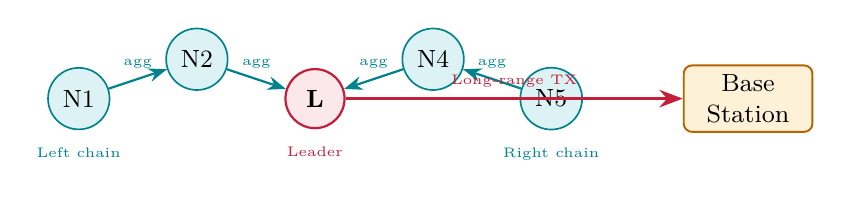
\begin{tikzpicture}[node distance=0.3cm,
  cnode/.style={circle, draw=myteal, fill=hdrteal, minimum size=0.75cm, font=\small, line width=0.6pt},
  lnode/.style={circle, draw=myred, fill=hdrred, minimum size=0.75cm, font=\small\bfseries, line width=0.8pt},
  bsnode/.style={rectangle, draw=myamber, fill=hdramber, text width=1.4cm, align=center, minimum height=0.75cm, font=\small, rounded corners=3pt, line width=0.7pt}]

  % Chain nodes
  \node[cnode] (n1) at (0,0)   {N1};
  \node[cnode] (n2) at (1.5,0.5) {N2};
  \node[lnode] (n3) at (3.0,0)  {L};
  \node[cnode] (n4) at (4.5,0.5) {N4};
  \node[cnode] (n5) at (6.0,0) {N5};
  \node[bsnode] (bs) at (8.5,0) {Base Station};

  % Chain links
  \draw[arrow, color=myteal] (n1) -- (n2) node[midway, above, font=\tiny] {agg};
  \draw[arrow, color=myteal] (n2) -- (n3) node[midway, above, font=\tiny] {agg};
  \draw[arrow, color=myteal] (n5) -- (n4) node[midway, above, font=\tiny] {agg};
  \draw[arrow, color=myteal] (n4) -- (n3) node[midway, above, font=\tiny] {agg};
  \draw[redarrow, line width=1.2pt] (n3) -- (bs) node[midway, above, font=\tiny, color=myred] {Long-range TX};

  \node[font=\tiny, color=myred, below=0.1cm of n3] {Leader};
  \node[font=\tiny, color=myteal, below=0.1cm of n1] {Left chain};
  \node[font=\tiny, color=myteal, below=0.1cm of n5] {Right chain};
\end{tikzpicture}
\end{tcolorbox}

\textbf{PEGASIS vs LEACH:}

\par\noindent
{\renewcommand{\arraystretch}{1.5}%
\begin{tabularx}{\linewidth}{|B{3.0cm}|Y|Y|}
\hline
\textbf{Parameter} & \textbf{LEACH} & \textbf{PEGASIS} \\
\hline
\textbf{Structure} & Clusters with CH & Single chain of all nodes \\
\hline
\textbf{Aggregation} & At CH only & Along entire chain (progressive) \\
\hline
\textbf{Transmission} & CH to BS (one-hop) & Leader to BS (one-hop) \\
\hline
\textbf{Energy balance} & Good (CH rotation) & Better (all nodes in chain share load) \\
\hline
\textbf{Latency} & Lower & Higher (data propagates along chain) \\
\hline
\textbf{Complexity} & Moderate & Higher (global chain construction) \\
\hline
\end{tabularx}}

\subsection{Data Aggregation and Fusion}

\begin{tcolorbox}[defbox, title={\textbf{Data Aggregation / Fusion --- Definition}}]
\textbf{Data aggregation} (also called \textbf{data fusion}) is the process of combining raw sensor readings from multiple nodes into a \textbf{single, compact, representative value} at an intermediate node (cluster head or relay) before forwarding to the base station. It reduces the volume of data transmitted, saving energy and bandwidth.
\end{tcolorbox}

\subsubsection*{Types of Data Aggregation}

\par\noindent
{\renewcommand{\arraystretch}{1.5}%
\begin{tabularx}{\linewidth}{|B{3.0cm}|Y|Y|}
\hline
\textbf{Type} & \textbf{Description} & \textbf{Example} \\
\hline
\textbf{Lossless aggregation} & Data combined without information loss & Concatenation, exact sum \\
\hline
\textbf{Lossy aggregation} & Data reduced with acceptable information loss & Average, max, min, median \\
\hline
\textbf{In-network processing} & Computation done at intermediate nodes, not just the sink & Cluster-head averaging in LEACH \\
\hline
\textbf{Suppression} & Nodes suppress transmission if reading is similar to a previous one (no change) & Temperature monitoring with dead-band \\
\hline
\end{tabularx}}

\subsubsection*{Common Aggregation Functions}
\begin{itemize}[leftmargin=*, itemsep=2pt]
  \item \textbf{MAX/MIN:} Forward the maximum or minimum of all received values. Used in intrusion detection.
  \item \textbf{SUM:} Total of all readings. Used in counting applications.
  \item \textbf{AVERAGE:} Mean of all readings. Used in temperature/environmental monitoring.
  \item \textbf{COUNT:} Number of nodes reporting. Used for density estimation.
  \item \textbf{Duplicate elimination:} Discard packets received from multiple paths with the same sequence number.
\end{itemize}

\textbf{Energy savings from aggregation:} If $k$ nodes each generate $b$ bits, naive forwarding requires $k \cdot b$ bits at the sink. Aggregating to a single message of $b$ bits reduces traffic by factor $k$ --- significant for large $k$.

% ===============================================================================
\section{Quality of a Sensor Network}
% ===============================================================================

\begin{tcolorbox}[formulabox, title={\textbf{QoS Metrics for WSN}}]
\begin{enumerate}[leftmargin=*, itemsep=5pt]
  \item \textbf{Energy efficiency / Network lifetime:} The most important metric. Lifetime = time until first (or $k$-th) node depletes its energy. Measured in hours or days.

  \item \textbf{Coverage:} Fraction of the monitored area where at least one sensor node can sense events. Full coverage $\Rightarrow$ every point in the field has a sensor within sensing radius $r_s$.

  \item \textbf{Connectivity:} The network is connected if there exists a path from every node to the sink. Requires $r_c \geq r_s$ (communication radius $\geq$ sensing radius).

  \item \textbf{Latency (Delay):} Time from event occurrence to data reaching the sink. Critical for real-time applications (fire detection, intruder alarm).

  \item \textbf{Reliability / Packet delivery ratio (PDR):} Fraction of generated data packets that are correctly received at the sink. $\text{PDR} = \frac{\text{received}}{\text{generated}}$

  \item \textbf{Data freshness:} How recent the received data is. Fresh data has small timestamp age.

  \item \textbf{Scalability:} Performance should degrade gracefully as node count increases from 10 to 10,000.

  \item \textbf{Fault tolerance:} Continued operation despite node or link failures.
\end{enumerate}
\end{tcolorbox}

\subsection{Real-Time Traffic Support in WSN}

Real-time applications (e.g., structural collapse detection, fire alarm) require end-to-end delay guarantees.

\begin{itemize}[leftmargin=*, itemsep=3pt]
  \item \textbf{Priority queuing:} High-priority (alarm) packets bypass normal queue.
  \item \textbf{Multi-path routing:} Maintain multiple paths; switch to backup on congestion.
  \item \textbf{Guaranteed Time Slots (GTS) in IEEE 802.15.4:} CFP slots are collision-free and schedule-based --- provides bounded latency.
  \item \textbf{SPEED protocol:} Stateless, geographic routing protocol designed for real-time traffic in WSN. Each node maintains a desired forwarding speed; if current speed is insufficient, the packet is re-routed.
  \item \textbf{Queue management:} Drop tail, RED (Random Early Detection), or priority-based scheduling at each relay node.
\end{itemize}

% ===============================================================================
\section{Security in Wireless Sensor Networks}
% ===============================================================================

WSN security is challenging because nodes are \textbf{physically exposed} in the field and have \textbf{very limited resources} for cryptographic computations.

\subsection{Security Goals (CIA + More)}

\begin{tcolorbox}[examplebox, title={\textbf{Security Goals in WSN}}]
\begin{itemize}[leftmargin=*, itemsep=4pt]
  \item \textbf{Confidentiality:} Only authorized parties can read the data. Achieved by symmetric encryption (AES).
  \item \textbf{Integrity:} Data is not modified in transit. Achieved by Message Authentication Codes (MAC).
  \item \textbf{Authentication:} Data genuinely comes from the claimed source. Achieved by keyed-hash MACs.
  \item \textbf{Availability:} The network remains operational despite attacks (anti-jamming, redundancy).
  \item \textbf{Freshness:} Data is recent, not a replay. Achieved by nonces, counters, or timestamps.
  \item \textbf{Self-organization:} Nodes can re-key and reform the network if a node is compromised.
\end{itemize}
\end{tcolorbox}

\subsection{Attack Types in WSN}

\par\noindent
{\renewcommand{\arraystretch}{1.5}%
\begin{tabularx}{\linewidth}{|B{3.0cm}|Y|Y|}
\hline
\textbf{Attack} & \textbf{Description} & \textbf{Defense} \\
\hline
\textbf{Sybil attack} & A malicious node presents multiple fake identities to the network & Identity-based authentication, physical challenge \\
\hline
\textbf{Wormhole attack} & Attacker tunnels packets between two distant points out-of-band, creating a fake short-cut & Geographic routing, TIK (time-based packet leash) \\
\hline
\textbf{Selective forwarding} & A malicious node drops selected packets instead of forwarding them all & Multi-path routing, ACK-based detection \\
\hline
\textbf{DoS (Jamming)} & Attacker transmits RF noise to block legitimate communication & Frequency hopping, spread spectrum (DSSS) \\
\hline
\textbf{Sinkhole attack} & A compromised node advertises a falsely attractive route to pull all traffic through itself & Geographic + authenticated routing \\
\hline
\textbf{Hello flood attack} & Attacker broadcasts HELLO packets with high power; distant nodes think it's a neighbor & Bidirectional link verification \\
\hline
\textbf{Replay attack} & Attacker captures a valid packet and retransmits it later & Timestamps, nonces, counters \\
\hline
\textbf{Node capture} & Physically capturing a node to extract keys & Key pre-distribution, threshold schemes \\
\hline
\end{tabularx}}

\subsection{SPINS: Security Protocols for Sensor Networks}

\begin{tcolorbox}[defbox, title={\textbf{SPINS --- Definition}}]
\textbf{SPINS (Security Protocols for Sensor Networks)} is a security framework for WSN that provides two building blocks:
\begin{itemize}
  \item \textbf{SNEP (Sensor Network Encryption Protocol):} Provides data confidentiality, data authentication, and data freshness between sensor nodes and base station.
  \item \textbf{\boldmath$\mu$TESLA (micro Timed Efficient Stream Loss-tolerant Authentication):} Provides \textbf{authenticated broadcast} from base station to sensor nodes using delayed key disclosure.
\end{itemize}
\end{tcolorbox}

\subsubsection*{SNEP Features}

\begin{itemize}[leftmargin=*, itemsep=3pt]
  \item Uses a shared symmetric key between each node and the base station (established at deployment).
  \item \textbf{Confidentiality:} Data encrypted with a block cipher (AES in counter mode).
  \item \textbf{Data authentication:} A MAC (Message Authentication Code) is appended to each message.
  \item \textbf{Freshness:} A counter (nonce) is included; base station checks that counter is monotonically increasing, preventing replay attacks.
  \item \textbf{Low overhead:} Counter is shared state; only 2 bytes added per packet for freshness (not a full timestamp).
\end{itemize}

\subsubsection*{\texorpdfstring{$\mu$}{mu}TESLA: Authenticated Broadcast}

Standard MACs require the receiver to share the key with the sender. In broadcast, if the key is shared with all receivers, any malicious receiver can forge messages. $\mu$TESLA solves this with \textbf{delayed key disclosure}:

\begin{enumerate}[leftmargin=*, itemsep=3pt]
  \item Base station generates a one-way key chain: $K_n, K_{n-1}, \ldots, K_1, K_0$ where $K_{i-1} = H(K_i)$ (hash function).
  \item Publishes commitment $K_0$ to all nodes at deployment.
  \item To broadcast a packet in time interval $i$: append MAC using $K_i$ (key not yet revealed).
  \item After the time interval passes, base station \textbf{discloses} $K_i$ to all nodes.
  \item Nodes verify the disclosed key (check $H(K_i) = K_{i-1}$) and then authenticate the buffered packet.
\end{enumerate}

\begin{tcolorbox}[tikzbox, title={\texorpdfstring{$\mu$}{mu}TESLA Key Chain and Delayed Disclosure}]
\centering
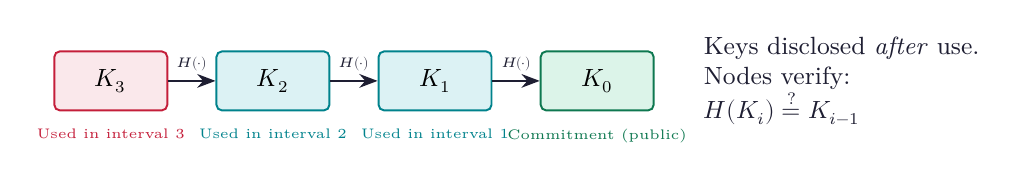
\begin{tikzpicture}[node distance=0.2cm,
  knode/.style={rectangle, draw=myteal, fill=hdrteal, text width=1.2cm, align=center, minimum height=0.75cm, font=\small\bfseries, rounded corners=2pt, line width=0.7pt}]

  \node[knode, fill=hdrred, draw=myred] (k3) {$K_3$};
  \node[knode, right=0.6cm of k3] (k2) {$K_2$};
  \node[knode, right=0.6cm of k2] (k1) {$K_1$};
  \node[knode, right=0.6cm of k1, fill=hdrgreen, draw=mygreen] (k0) {$K_0$};

  \draw[arrow] (k3) -- (k2) node[midway, above, font=\tiny] {$H(\cdot)$};
  \draw[arrow] (k2) -- (k1) node[midway, above, font=\tiny] {$H(\cdot)$};
  \draw[arrow] (k1) -- (k0) node[midway, above, font=\tiny] {$H(\cdot)$};

  \node[font=\tiny, color=myred, below=0.1cm of k3] {Used in interval 3};
  \node[font=\tiny, color=myteal, below=0.1cm of k2] {Used in interval 2};
  \node[font=\tiny, color=myteal, below=0.1cm of k1] {Used in interval 1};
  \node[font=\tiny, color=mygreen, below=0.1cm of k0] {Commitment (public)};

  \node[right=0.5cm of k0, font=\small, color=mydark, align=left]
    {Keys disclosed \textit{after} use.\\ Nodes verify:\\$H(K_i) \stackrel{?}{=} K_{i-1}$};
\end{tikzpicture}
\end{tcolorbox}

\subsection{Key Management in WSN}

\begin{itemize}[leftmargin=*, itemsep=3pt]
  \item \textbf{Pre-deployment key loading:} Each node gets a unique secret key shared with the base station.
  \item \textbf{Random key pre-distribution (Eschenauer-Gligor):} Each node pre-loaded with a random subset of keys from a large key pool. Two neighboring nodes likely share at least one key (used for pairwise link encryption).
  \item \textbf{Threshold-based schemes:} A secret key is split into $n$ shares using Shamir's Secret Sharing; any $k$ out of $n$ nodes can reconstruct the key.
\end{itemize}

% ===============================================================================
\newpage
\section{Quick Revision --- Module 4}
% ===============================================================================

\begin{tcolorbox}[formulabox, title={\textbf{Key Formulas and Metrics at a Glance}}]
\begin{itemize}[leftmargin=*, itemsep=4pt]
  \item PDR (Packet Delivery Ratio): $\text{PDR} = \dfrac{\text{Packets received at sink}}{\text{Packets generated at source}} \times 100\%$
  \item Network lifetime: $T = \min_i \left(\dfrac{E_i}{P_i}\right)$ (limited by first node to die)
  \item Coverage: $C = \dfrac{\text{Sensed area}}{\text{Total monitored area}}$; per-node sensing area $= \pi r_s^2$
  \item Energy saved by aggregation: $E_{\text{saved}} = (k-1) \times b \times E_{\text{tx/bit}}$ for $k$ nodes aggregated
  \item $\mu$TESLA key chain: $K_{i-1} = H(K_i)$, verify: $H(K_{\text{disclosed}}) = K_{\text{prev}}$
\end{itemize}
\end{tcolorbox}

\begin{tcolorbox}[defbox, title={\textbf{One-Line Definitions}}]
\begin{itemize}[leftmargin=*, itemsep=3pt]
  \item \textbf{Data dissemination:} Propagating data or queries across WSN from source to destination with energy efficiency.
  \item \textbf{Rumor routing:} Agents wander creating routing tables; queries find event by intersecting agent trails.
  \item \textbf{PEGASIS:} Chain-based data gathering; data aggregated node-by-node to leader, then to base station.
  \item \textbf{Data aggregation:} Combining multiple sensor readings into a single compact value to save transmission energy.
  \item \textbf{Sybil attack:} Malicious node uses multiple fake identities to influence routing or voting.
  \item \textbf{Wormhole attack:} Attacker tunnels packets out-of-band to create a false short-cut route.
  \item \textbf{SPINS:} Security framework for WSN comprising SNEP (confidentiality/authentication) and $\mu$TESLA (authenticated broadcast).
  \item \textbf{$\mu$TESLA:} Authenticated broadcast via delayed key disclosure from a one-way key chain.
\end{itemize}
\end{tcolorbox}

\begin{tcolorbox}[exambox, title={\textbf{Frequently Asked / Viva Questions --- Module 4}}]
\begin{enumerate}[leftmargin=*, itemsep=5pt]
  \item \Q{What is data dissemination in WSN? Name two dissemination protocols.}
  Data dissemination is the mechanism by which data or queries are propagated across the WSN from source to sinks (or vice versa) efficiently. Two protocols: (1) \textbf{Directed Diffusion} --- interest flooding, gradient setup, data delivery; (2) \textbf{Rumor Routing} --- agents propagate from event sources; queries find events by intersecting agent trails.

  \item \Q{Explain data aggregation in WSN. What are its benefits?}
  Data aggregation combines sensor readings from multiple nodes into a single compact value at an intermediate node before forwarding to the sink. Benefits: (1) Reduces data volume $\Rightarrow$ fewer transmissions $\Rightarrow$ energy savings; (2) Reduces congestion; (3) Eliminates redundant data from correlated sensors.

  \item \Q{What is PEGASIS? How is it better than LEACH?}
  PEGASIS (Power-Efficient GAthering in Sensor Information Systems) forms a single chain of all nodes; data is aggregated along the chain to a rotating leader that transmits to the base station. Better than LEACH because: (1) Progressive in-network aggregation reduces total data volume; (2) Each node only communicates with its nearest neighbor (shorter range $\Rightarrow$ less energy); (3) Leader rotation distributes the high-energy BS transmission among all nodes.

  \item \Q{List four QoS metrics for a wireless sensor network.}
  (1) \textbf{Network lifetime} --- time until first node dies; (2) \textbf{Coverage} --- fraction of area monitored; (3) \textbf{Latency} --- delay from event to sink; (4) \textbf{PDR (Packet Delivery Ratio)} --- fraction of packets successfully received.

  \item \Q{What is the Sybil attack and how is it prevented?}
  In a Sybil attack, a malicious node presents multiple fake identities to the network, allowing it to manipulate routing decisions, vote-based algorithms, or reputation systems. Prevention: (1) Identity-based authentication (each node has a unique certificate); (2) Physical challenge tests (test if a ``node'' is actually at its claimed location); (3) Radio fingerprinting.

  \item \Q{Explain the wormhole attack and its impact on WSN.}
  Two colluding attackers at distant parts of the network create a private, out-of-band tunnel (wormhole). Packets received by one end are instantly forwarded to the other end, making distant nodes appear as neighbors. This distorts routing: nodes route via the wormhole (thinking it is a short path), allowing attackers to eavesdrop or drop packets. Countermeasures: TIK (timestamp-based packet leash), geographic routing with location verification.

  \item \Q{What is SPINS? Explain SNEP.}
  SPINS (Security Protocols for Sensor Networks) provides two security primitives. \textbf{SNEP} (Sensor Network Encryption Protocol) provides: confidentiality (AES counter-mode encryption), data authentication (keyed MAC), and freshness (shared counter prevents replay). Low overhead: only 8 bytes MAC per packet. SNEP uses pairwise shared keys between each node and the base station.

  \item \Q{How does $\mu$TESLA provide authenticated broadcast?}
  $\mu$TESLA uses a \textbf{one-way key chain}: $K_{i-1} = H(K_i)$, bootstrapped with commitment $K_0$ published to all nodes. For interval $i$, base station authenticates broadcast with $K_i$ (key still secret). After the interval ends, $K_i$ is disclosed. Nodes verify: $H(K_i) \stackrel{?}{=} K_{i-1}$. If valid, they authenticate the earlier buffered message. Delayed disclosure ensures receivers cannot forge the MAC.

  \item \Q{What is selective forwarding attack in WSN?}
  A malicious intermediate node drops specific packets instead of forwarding them all. It behaves correctly for some flows to avoid detection. Impact: data loss, reduced PDR, silent disruption of critical sensor data. Defense: multi-path routing ensures data reaches sink via alternative paths; ACK-based detection flags suspicious forwarders.

  \item \Q{What is real-time traffic support in WSN?}
  Applications like fire alarms or structural collapse detection require end-to-end delay guarantees. Mechanisms: (1) \textbf{Priority queuing} at routers for alarm packets; (2) \textbf{GTS slots} in IEEE 802.15.4 (collision-free, bounded delay); (3) \textbf{SPEED protocol} --- geographic routing enforcing minimum forwarding speed; (4) Multi-path routing for congestion avoidance.

  \item \Q{Differentiate data gathering and data dissemination.}
  \textbf{Data gathering} = collecting sensor readings from nodes to the base station (many-to-one, uplink). \textbf{Data dissemination} = propagating queries or commands from sink to sensor nodes, or flooding data from a source to multiple sinks (one-to-many or controlled spreading). Gathering protocols: PEGASIS, LEACH. Dissemination protocols: Directed Diffusion, Rumor Routing, SPIN.

  \item \Q{What is the Hello flood attack?}
  An attacker with a powerful radio broadcasts HELLO messages at high power. Nodes far away hear this and assume the attacker is a one-hop neighbor, establishing routes through it. When they try to send data via this ``neighbor,'' packets are lost or intercepted. Defense: bidirectional link verification --- a node only considers a neighbor if it can receive a reply from that neighbor at normal power.
\end{enumerate}
\end{tcolorbox}

\begin{tcolorbox}[tikzbox, title={\textbf{Summary: WSN Security Threats and Countermeasures}}]
\par\noindent
{\renewcommand{\arraystretch}{1.4}%
\begin{tabularx}{\linewidth}{|B{2.8cm}|Y|Y|}
\hline
\textbf{Attack} & \textbf{Layer} & \textbf{Countermeasure} \\
\hline
Sybil & Network & Identity auth., radio fingerprint \\
\hline
Wormhole & Network & Packet leash (TIK), location verify \\
\hline
Selective forward & Network & Multi-path, ACK detection \\
\hline
DoS / Jamming & Physical & DSSS, frequency hopping \\
\hline
Replay & MAC/Net & Nonce, timestamp, counter (SNEP) \\
\hline
Hello flood & Network & Bidirectional link verification \\
\hline
Node capture & Physical & Key pre-distribution, threshold \\
\hline
\end{tabularx}}
\end{tcolorbox}


% -- Module 5 -----------------------------------------------------------------
\modulestart{5}{Design Principles for Wireless Sensor Networks}

\section{Design Principles for Wireless Sensor Networks}
% ===============================================================================

WSN design is fundamentally different from traditional network design. The scarcity of energy, computation, and memory requires application-aware, cross-layer, and energy-first design principles.

\begin{tcolorbox}[formulabox, title={\textbf{Core WSN Design Principles}}]
\begin{enumerate}[leftmargin=*, itemsep=5pt]
  \item \textbf{Energy efficiency first:} Every design decision --- protocol, algorithm, hardware --- must minimize energy consumption. Network lifetime is the primary performance metric. Aggressive duty cycling (radio sleep), in-network processing, and shortest-path routing are non-negotiable.

  \item \textbf{In-network processing (data-centric design):} Perform aggregation, filtering, and fusion inside the network, not just at the sink. A cluster head that averages 10 readings saves $9\times$ the transmission energy of forwarding raw data.

  \item \textbf{Cross-layer design:} Traditional layered (OSI) design isolates layers. WSN protocols jointly optimize MAC + routing + application (e.g., LEACH combines clustering at the network layer with TDMA at the MAC layer, driven by application data rate).

  \item \textbf{Self-organization and adaptivity:} The network must configure itself, elect cluster heads, discover routes, and heal from failures without human intervention. Protocols must work correctly under random deployment and topology changes.

  \item \textbf{Collaboration and redundancy:} Exploit spatial redundancy --- multiple nodes cover the same area. Use data from multiple sensors for reliability and accuracy (spatial diversity). Active nodes can cover for sleeping or dead nodes.

  \item \textbf{Data-centric communication:} Address data by its attributes (``temperature $> 40$°C''), not by node IDs. This enables in-network aggregation, suppression of duplicate data, and semantic routing.

  \item \textbf{Quality/fidelity trade-off:} Accept lower resolution or less frequent data in exchange for energy savings. Adaptive sampling reduces data rate when environment is stable, increases it during events.

  \item \textbf{Security by design:} Assume a hostile deployment environment. Build authentication and freshness into every protocol (not bolted on after). Use lightweight symmetric cryptography (AES-128) rather than public-key.
\end{enumerate}
\end{tcolorbox}

% ===============================================================================
\section{Gateway Concepts in WSN}
% ===============================================================================

\begin{tcolorbox}[defbox, title={\textbf{WSN Gateway --- Definition}}]
A \textbf{WSN gateway} is a device that bridges the wireless sensor network with an external network (such as the Internet, an enterprise LAN, or a cellular network). It performs \textbf{protocol translation} between the low-power WSN protocols (IEEE 802.15.4 / ZigBee) and standard IP networking (TCP/IP / HTTP).
\end{tcolorbox}

\subsection{Need for a Gateway}

\begin{itemize}[leftmargin=*, itemsep=3pt]
  \item WSN nodes speak IEEE 802.15.4 / ZigBee; the internet speaks TCP/IP. These are incompatible at multiple layers.
  \item Sensor nodes are too resource-constrained to run a full TCP/IP stack.
  \item The gateway provides a management interface for the WSN (task injection, firmware update, health monitoring).
  \item The gateway buffers data from the WSN and forwards to cloud/server in bursts, reducing WSN active time.
\end{itemize}

\subsection{Gateway Architecture and Functions}

\begin{tcolorbox}[tikzbox, title={WSN Gateway Integration Diagram}]
\centering
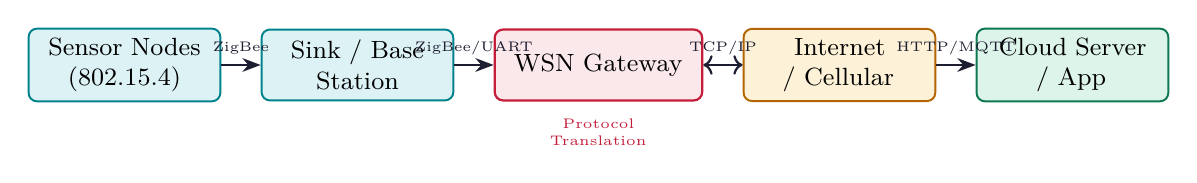
\begin{tikzpicture}[node distance=0.5cm and 0.9cm,
  wsblock/.style={rectangle, draw=myteal, fill=hdrteal, text width=2.2cm,
    align=center, minimum height=0.9cm, font=\small, rounded corners=3pt, line width=0.7pt},
  gwblock/.style={rectangle, draw=myred, fill=hdrred, text width=2.4cm,
    align=center, minimum height=0.9cm, font=\small, rounded corners=3pt, line width=0.8pt},
  ipblock/.style={rectangle, draw=myamber, fill=hdramber, text width=2.2cm,
    align=center, minimum height=0.9cm, font=\small, rounded corners=3pt, line width=0.7pt},
  srvblock/.style={rectangle, draw=mygreen, fill=hdrgreen, text width=2.2cm,
    align=center, minimum height=0.9cm, font=\small, rounded corners=3pt, line width=0.7pt}]

  % WSN side
  \node[wsblock] (sn) {Sensor Nodes (802.15.4)};
  \node[wsblock, right=0.5cm of sn] (sink) {Sink / Base Station};

  % Gateway
  \node[gwblock, right=0.5cm of sink] (gw) {WSN Gateway};

  % Internet
  \node[ipblock, right=0.5cm of gw] (inet) {Internet / Cellular};

  % Server / Cloud
  \node[srvblock, right=0.5cm of inet] (srv) {Cloud Server / App};

  % Arrows
  \draw[arrow] (sn) -- (sink) node[midway, above, font=\tiny] {ZigBee};
  \draw[arrow] (sink) -- (gw) node[midway, above, font=\tiny] {ZigBee/UART};
  \draw[arrow, <->] (gw) -- (inet) node[midway, above, font=\tiny] {TCP/IP};
  \draw[arrow] (inet) -- (srv) node[midway, above, font=\tiny] {HTTP/MQTT};

  % Gateway label
  \node[font=\tiny, color=myred, below=0.1cm of gw, align=center, text width=1.8cm] {Protocol Translation};
\end{tikzpicture}
\end{tcolorbox}

\textbf{Gateway functions:}
\begin{itemize}[leftmargin=*, itemsep=3pt]
  \item \textbf{Protocol translation:} Converts ZigBee/IEEE 802.15.4 frames to IP packets and vice versa.
  \item \textbf{Data buffering:} Stores sensor data locally (flash/SD card) if internet is unavailable.
  \item \textbf{Data formatting:} Converts raw sensor values to JSON, XML, or MQTT payloads for cloud APIs.
  \item \textbf{Security bridging:} Translates between WSN security (AES-128 with SNEP) and internet security (TLS/SSL).
  \item \textbf{Task injection:} Receives queries from the internet and injects them as interests into the WSN.
  \item \textbf{Network management:} Monitors WSN health, tracks node battery levels, and triggers alarms.
\end{itemize}

% ===============================================================================
\section{WSN to Internet Communication}
% ===============================================================================

\begin{tcolorbox}[defbox, title={\textbf{WSN-to-Internet Communication}}]
\textbf{WSN to Internet} communication refers to the uplink flow where sensor data is transported from the sensor field, through the gateway, to an Internet-connected server or cloud platform for storage, processing, and visualization.
\end{tcolorbox}

\subsection{Integration Approaches}

\par\noindent
{\renewcommand{\arraystretch}{1.5}%
\begin{tabularx}{\linewidth}{|B{3.2cm}|Y|Y|}
\hline
\textbf{Approach} & \textbf{Description} & \textbf{Protocols} \\
\hline
\textbf{Gateway-based (Overlay)} & WSN and Internet are two separate networks; gateway translates between them & ZigBee + HTTP/MQTT gateway \\
\hline
\textbf{6LoWPAN (IP-native)} & Runs IPv6 directly on IEEE 802.15.4 nodes using header compression; no separate gateway needed & 6LoWPAN + CoAP + RPL \\
\hline
\textbf{Middleware approach} & Software layer abstracts WSN heterogeneity; presents a uniform API to internet applications & REST-based middleware \\
\hline
\end{tabularx}}

\subsection{6LoWPAN (IPv6 over Low-Power Wireless PANs)}

\begin{tcolorbox}[defbox, title={\textbf{6LoWPAN --- Definition}}]
\textbf{6LoWPAN} is an IETF adaptation layer (RFC 4944) that enables \textbf{IPv6 packets to be transmitted over IEEE 802.15.4} networks by compressing IPv6 headers (from 40 bytes to 2--6 bytes) and fragmenting large packets to fit the 127-byte IEEE 802.15.4 frame. This allows sensor nodes to participate directly in the Internet of Things.
\end{tcolorbox}

\textbf{Key functions of 6LoWPAN adaptation layer:}
\begin{itemize}[leftmargin=*, itemsep=3pt]
  \item \textbf{Header compression:} IPv6 header (40 B) + UDP (8 B) compressed to $\leq$ 6 B using IPHC (IP Header Compression).
  \item \textbf{Fragmentation and reassembly:} IPv6 MTU = 1280 B; IEEE 802.15.4 payload = 102 B (max). 6LoWPAN fragments and reassembles.
  \item \textbf{Mesh addressing:} Supports multi-hop routing for IEEE 802.15.4 using mesh header.
  \item \textbf{Neighbor discovery:} Optimized ND for low-power, lossy networks (ND-LowPAN).
\end{itemize}

\subsection{CoAP (Constrained Application Protocol)}

\begin{tcolorbox}[defbox, title={\textbf{CoAP --- Definition}}]
\textbf{CoAP} is a lightweight application protocol designed for constrained IoT and WSN devices, functioning as the ``HTTP for IoT.'' It runs over UDP (instead of TCP), uses a REST-based request/response model, and supports GET, PUT, POST, DELETE operations on resources (sensor readings, actuator states).
\end{tcolorbox}

\begin{itemize}[leftmargin=*, itemsep=3pt]
  \item \textbf{Binary encoding:} Compact binary header (4 bytes fixed header vs HTTP's 100s of bytes).
  \item \textbf{UDP-based:} Avoids TCP's connection overhead and handshake energy cost.
  \item \textbf{Confirmable messages:} CoAP has its own reliability mechanism (CON messages with ACK).
  \item \textbf{Observe extension:} Server pushes updates to subscribed clients (no polling needed).
  \item \textbf{Gateway translation:} A CoAP-HTTP proxy converts between CoAP (sensor side) and HTTP (internet side).
\end{itemize}

% ===============================================================================
\section{Internet to WSN Communication}
% ===============================================================================

\begin{tcolorbox}[defbox, title={\textbf{Internet-to-WSN Communication}}]
\textbf{Internet to WSN} communication refers to the downlink flow: queries, commands, firmware updates, and configuration sent from an Internet-connected server or user application into the sensor network.
\end{tcolorbox}

\subsection{Challenges of Internet-to-WSN Downlink}
\begin{itemize}[leftmargin=*, itemsep=3pt]
  \item \textbf{Sleeping nodes:} Sensor nodes may be asleep when a command arrives. The gateway must buffer the command and deliver it at the node's next wake-up.
  \item \textbf{Asymmetric bandwidth:} Internet downlink can push data faster than the WSN can absorb.
  \item \textbf{Addressing:} Individual nodes may have only 16-bit short addresses (not globally routable). The gateway maps external requests to internal WSN addresses.
  \item \textbf{Reliability:} IEEE 802.15.4 is lossy; downlink commands may need retransmission.
\end{itemize}

\subsection{Mechanisms}
\begin{itemize}[leftmargin=*, itemsep=3pt]
  \item \textbf{MQTT (Message Queuing Telemetry Transport):} Publish-subscribe protocol over TCP; the broker buffers messages for offline sensor nodes. Gateway subscribes to topics and injects commands into WSN.
  \item \textbf{RPL (Routing Protocol for Low-Power and Lossy Networks):} IETF routing protocol for 6LoWPAN; builds a Destination-Oriented DAG (DODAG) from the sink downward, enabling Internet-initiated routes.
  \item \textbf{CoAP Observe:} Internet server registers observation on a sensor resource; sensor pushes updates. Reverse: server PUTs commands to sensor actuator resources.
\end{itemize}

% ===============================================================================
\section{Operating Systems for WSN}
% ===============================================================================

\begin{tcolorbox}[defbox, title={\textbf{WSN Operating System --- Requirements}}]
An \textbf{embedded OS for WSN} must: fit in $< 10$ KB RAM and $< 100$ KB Flash, support concurrent tasks (sensing, routing, communication) on a single MCU, manage radio duty cycling, provide hardware abstraction for different sensor platforms, and be energy-aware (support for sleep modes).
\end{tcolorbox}

\subsection{Comparison: WSN OS vs General-Purpose OS}

\par\noindent
{\renewcommand{\arraystretch}{1.5}%
\begin{tabularx}{\linewidth}{|B{3.0cm}|Y|Y|}
\hline
\textbf{Feature} & \textbf{General-Purpose OS (Linux)} & \textbf{WSN OS (TinyOS)} \\
\hline
\textbf{RAM footprint} & 10s of MB & 2--10 KB \\
\hline
\textbf{Flash/ROM} & 100s of MB & 30--100 KB \\
\hline
\textbf{Scheduling model} & Preemptive multi-threading & Event-driven (non-preemptive) \\
\hline
\textbf{Energy management} & Limited & First-class: radio, CPU sleep control \\
\hline
\textbf{Hardware abstraction} & Device drivers, system calls & Component interfaces (nesC) \\
\hline
\textbf{Process isolation} & Yes (MMU) & No MMU; single address space \\
\hline
\textbf{Concurrency} & Full multi-process/thread & Events + tasks (split-phase) \\
\hline
\end{tabularx}}

% ===============================================================================
\section{TinyOS}
% ===============================================================================

\begin{tcolorbox}[defbox, title={\textbf{TinyOS --- Definition}}]
\textbf{TinyOS} is an open-source, \textbf{event-driven} operating system designed for resource-constrained sensor network nodes. Developed at UC Berkeley (2000), it is implemented in \textbf{nesC} and uses a \textbf{component-based architecture} where applications are assembled from reusable hardware and software components.
\end{tcolorbox}

\subsection{Key Features of TinyOS}

\begin{itemize}[leftmargin=*, itemsep=3pt]
  \item \textbf{Event-driven model:} No blocking calls. All long-running operations are \textbf{split-phase}: operation is started with a \textit{command}, and its completion triggers an \textit{event}.
  \item \textbf{Small footprint:} Core TinyOS $< 400$ bytes. Entire system with a basic radio stack fits in $<$ 15 KB Flash.
  \item \textbf{Component-based:} Applications are composed of \textbf{components} that communicate through \textbf{interfaces}. No dynamic linking.
  \item \textbf{Two-level concurrency:} \textbf{Events} (hardware interrupts, split-phase completions) run at high priority; \textbf{Tasks} (deferred computation) run in FIFO order at lower priority.
  \item \textbf{Compile-time configuration:} Component wiring is done at compile time (by the developer using a ``wiring'' file), not at runtime. This removes overhead of runtime dynamic dispatch.
  \item \textbf{TinyOS scheduler:} Single FIFO task queue. Events can interrupt tasks. Tasks run to completion (non-preemptive).
\end{itemize}

\begin{tcolorbox}[tikzbox, title={TinyOS Component Model}]
\centering
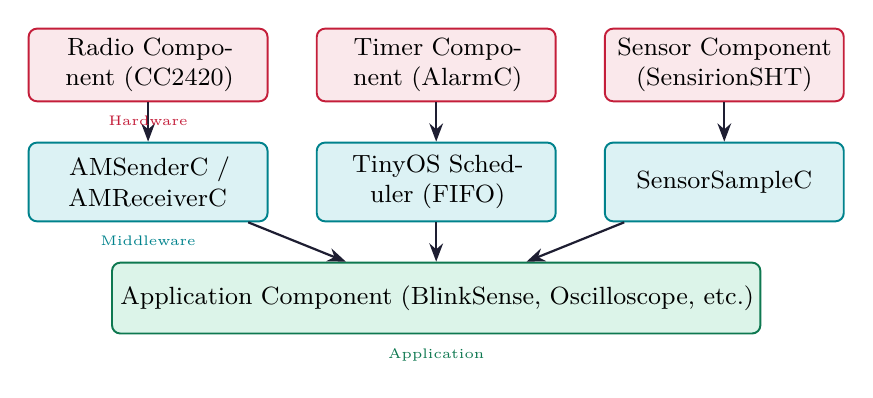
\begin{tikzpicture}[node distance=0.5cm and 0.9cm,
  comp/.style={rectangle, draw=myteal, fill=hdrteal, text width=2.8cm,
    align=center, minimum height=1.0cm, font=\small, rounded corners=3pt, line width=0.7pt},
  hwcomp/.style={rectangle, draw=myred, fill=hdrred, text width=2.8cm,
    align=center, minimum height=0.9cm, font=\small, rounded corners=3pt, line width=0.7pt},
  appcomp/.style={rectangle, draw=mygreen, fill=hdrgreen, text width=2.8cm,
    align=center, minimum height=0.9cm, font=\small, rounded corners=3pt, line width=0.7pt}]

  % Hardware components
  \node[hwcomp] (radio) {Radio Component (CC2420)};
  \node[hwcomp, right=0.6cm of radio] (timer) {Timer Component (AlarmC)};
  \node[hwcomp, right=0.6cm of timer] (sens) {Sensor Component (SensirionSHT)};

  % Middleware / OS
  \node[comp, below=0.5cm of radio] (mac) {AMSenderC / AMReceiverC};
  \node[comp, below=0.5cm of timer] (sched) {TinyOS Scheduler (FIFO)};
  \node[comp, below=0.5cm of sens] (sample) {SensorSampleC};

  % Application
  \node[appcomp, below=0.5cm of sched, text width=8cm] (app) {Application Component (BlinkSense, Oscilloscope, etc.)};

  % Connections
  \draw[arrow] (radio) -- (mac);
  \draw[arrow] (timer) -- (sched);
  \draw[arrow] (sens) -- (sample);
  \draw[arrow] (mac) -- (app);
  \draw[arrow] (sched) -- (app);
  \draw[arrow] (sample) -- (app);

  \node[font=\tiny, color=myred, below=0.05cm of radio] {Hardware};
  \node[font=\tiny, color=myteal, below=0.05cm of mac] {Middleware};
  \node[font=\tiny, color=mygreen, below=0.05cm of app] {Application};
\end{tikzpicture}
\end{tcolorbox}

% ===============================================================================
\section{nesC Programming Language}
% ===============================================================================

\begin{tcolorbox}[defbox, title={\textbf{nesC --- Definition}}]
\textbf{nesC} (network embedded systems C) is a component-based, event-driven extension of the C programming language designed specifically for TinyOS and sensor network applications. It provides the \textbf{component model}, \textbf{interface} declarations, and \textbf{wiring} syntax to compose TinyOS applications from reusable modules.
\end{tcolorbox}

\subsection{Key nesC Concepts}

\subsubsection*{1. Interfaces}
An \textbf{interface} defines a set of bidirectional operations:
\begin{itemize}[leftmargin=*, itemsep=2pt]
  \item \textbf{Commands:} Called by the user of the interface (top-down call). E.g., \texttt{AMSend.send()}.
  \item \textbf{Events:} Signaled by the provider of the interface (bottom-up notification). E.g., \texttt{AMSend.sendDone()}.
\end{itemize}

\subsubsection*{2. Components}
Two types of components:
\begin{itemize}[leftmargin=*, itemsep=2pt]
  \item \textbf{Module:} Implements an interface; contains C-like code for commands and event handlers.
  \item \textbf{Configuration:} Wires components together (no code, only connections).
\end{itemize}

\subsubsection*{3. Split-Phase Operations}
Long-running operations (radio TX, ADC conversion) are split into:
\begin{itemize}[itemsep=2pt]
  \item \textbf{Initiation:} Call a command (e.g., \texttt{call AMSend.send(...)}) --- returns immediately.
  \item \textbf{Completion:} An event is signaled when done (e.g., \texttt{event AMSend.sendDone(...)}). No blocking.
\end{itemize}

\subsubsection*{4. Tasks}
\begin{itemize}[itemsep=2pt]
  \item Deferred computation: \texttt{post myTask();} schedules a task in the FIFO queue.
  \item Tasks run to completion; they cannot be preempted by other tasks (only by events/interrupts).
\end{itemize}

\subsubsection*{5. Atomicity and Race Conditions}
\begin{itemize}[itemsep=2pt]
  \item \texttt{atomic \{ ... \}} block: disables interrupts for short, critical sections.
  \item nesC compiler performs a \textbf{race condition analysis} at compile time to flag potential data races between tasks and events.
\end{itemize}

\subsection{TinyOS vs Linux vs RTOS}

\par\noindent
{\renewcommand{\arraystretch}{1.5}%
\begin{tabularx}{\linewidth}{|B{2.8cm}|Y|Y|Y|}
\hline
\textbf{Feature} & \textbf{TinyOS} & \textbf{Linux} & \textbf{RTOS (FreeRTOS)} \\
\hline
\textbf{RAM} & 2--10 KB & 10s MB & 5--50 KB \\
\hline
\textbf{Scheduling} & Event-driven & Preemptive & Preemptive \\
\hline
\textbf{Tasks} & FIFO, non-preemptive & Preemptable threads & Priority-based tasks \\
\hline
\textbf{Language} & nesC (C extension) & C & C \\
\hline
\textbf{Energy mgmt} & First-class & Limited & Good \\
\hline
\textbf{Blocking calls} & Not allowed & Allowed & Allowed \\
\hline
\textbf{Use case} & WSN motes (8/16-bit MCU) & General-purpose (Raspberry Pi) & IoT/embedded (ARM Cortex-M) \\
\hline
\end{tabularx}}

% ===============================================================================
\newpage
\section{Quick Revision --- Module 5}
% ===============================================================================

\begin{tcolorbox}[formulabox, title={\textbf{Key Concepts at a Glance}}]
\begin{itemize}[leftmargin=*, itemsep=4pt]
  \item 6LoWPAN header compression: IPv6 (40 B) + UDP (8 B) $\rightarrow$ IPHC compressed header ($\leq$ 6 B)
  \item IEEE 802.15.4 max payload: 127 B (PHY), 102 B (MAC, after headers)
  \item IPv6 MTU: 1280 B $\Rightarrow$ 6LoWPAN fragmentation required
  \item CoAP fixed header: only 4 bytes (vs HTTP $>$ 100 bytes)
  \item TinyOS scheduler: FIFO task queue; non-preemptive tasks; events interrupt tasks
  \item nesC split-phase: \texttt{call Iface.start()} initiates; \texttt{event Iface.startDone()} signals completion
  \item Gateway function: Protocol translation (ZigBee $\leftrightarrow$ TCP/IP), buffering, security bridging
\end{itemize}
\end{tcolorbox}

\begin{tcolorbox}[defbox, title={\textbf{One-Line Definitions}}]
\begin{itemize}[leftmargin=*, itemsep=3pt]
  \item \textbf{WSN Gateway:} Bridges IEEE 802.15.4/ZigBee WSN to Internet via protocol translation and data formatting.
  \item \textbf{6LoWPAN:} IETF adaptation layer running IPv6 over IEEE 802.15.4 via header compression and fragmentation.
  \item \textbf{CoAP:} Lightweight REST protocol over UDP for constrained IoT devices; the ``HTTP of IoT.''
  \item \textbf{RPL:} IETF routing protocol for 6LoWPAN; builds a DODAG (Destination-Oriented DAG) for uplink and downlink routing.
  \item \textbf{MQTT:} Publish-subscribe message protocol over TCP; broker buffers messages for offline sensor nodes.
  \item \textbf{TinyOS:} Event-driven, component-based OS for sensor motes; $<$15 KB footprint; non-preemptive.
  \item \textbf{nesC:} System programming language for TinyOS; extends C with components, interfaces, and wiring.
  \item \textbf{Split-phase:} Operation model where a command initiates and an event signals completion; no blocking.
\end{itemize}
\end{tcolorbox}

\begin{tcolorbox}[exambox, title={\textbf{Frequently Asked / Viva Questions --- Module 5}}]
\begin{enumerate}[leftmargin=*, itemsep=5pt]
  \item \Q{What are the key design principles for WSN?}
  Eight principles: (1) Energy efficiency first; (2) In-network processing/aggregation; (3) Cross-layer design; (4) Self-organization and adaptivity; (5) Collaboration and redundancy; (6) Data-centric communication; (7) Quality/fidelity trade-off; (8) Security by design. Energy is always the primary constraint driving all design decisions.

  \item \Q{What is a WSN gateway? What are its functions?}
  A WSN gateway bridges the sensor network (IEEE 802.15.4/ZigBee) to the Internet. Functions: (1) Protocol translation (ZigBee $\leftrightarrow$ TCP/IP); (2) Data buffering; (3) Data formatting (JSON/MQTT); (4) Security bridging (WSN AES $\leftrightarrow$ internet TLS); (5) Task/query injection into WSN; (6) Network management and monitoring.

  \item \Q{What is 6LoWPAN? Why is it needed?}
  6LoWPAN (IPv6 over Low-Power WPANs) is an adaptation layer (RFC 4944) enabling IPv6 packets to run over IEEE 802.15.4. It is needed because: IPv6 header = 40 B but 802.15.4 payload = 102 B (only 62 B left for UDP+data after raw IPv6). 6LoWPAN compresses IPv6+UDP to $\leq$ 6 B using IPHC and fragments large packets, enabling IP-native WSN nodes.

  \item \Q{What is CoAP? How does it differ from HTTP?}
  CoAP (Constrained Application Protocol) is a lightweight REST protocol for IoT running over UDP. Differences from HTTP: runs over UDP (not TCP), has only 4-byte fixed header (vs 100+ bytes in HTTP), uses binary encoding (not text), includes built-in reliability (CON/ACK), supports observe mode (server push). Designed for $< 10$ KB RAM devices.

  \item \Q{Explain TinyOS architecture.}
  TinyOS is an event-driven, component-based OS. Architecture: (1) \textbf{Components} --- modules (implement code) and configurations (wire components); (2) \textbf{Interfaces} --- define commands (calls) and events (callbacks); (3) \textbf{Scheduler} --- FIFO task queue; tasks run to completion; events can interrupt tasks; (4) \textbf{Split-phase} --- no blocking calls; operations initiated by commands, completed by events. Footprint: $<$15 KB Flash, $<$4 KB RAM.

  \item \Q{What is nesC? Explain its key concepts.}
  nesC (network embedded systems C) is a component-based C extension for TinyOS. Key concepts: (1) \textbf{Interface} --- defines commands (top-down) and events (bottom-up); (2) \textbf{Module} --- implements an interface; (3) \textbf{Configuration} --- wires components at compile time; (4) \textbf{Split-phase} --- non-blocking; (5) \textbf{Tasks} --- deferred computation posted to FIFO queue; (6) \textbf{Atomic} --- interrupt-disable for race-condition-free critical sections.

  \item \Q{What is a split-phase operation in TinyOS? Give an example.}
  A split-phase operation separates initiation from completion: the call initiates an operation and returns immediately (no blocking); an event fires when the operation is done. Example: \texttt{call AMSend.send(msg)} starts radio transmission and returns immediately. When TX is done, \texttt{event AMSend.sendDone(msg, error)} is triggered for the application to handle success/failure.

  \item \Q{Compare TinyOS, Linux, and FreeRTOS for WSN use.}
  TinyOS: 2--10 KB RAM, event-driven, FIFO non-preemptive tasks, designed for 8/16-bit WSN motes. Linux: 10s MB RAM, preemptive threads, general-purpose, too heavy for motes. FreeRTOS: 5--50 KB RAM, preemptive priority tasks, good energy management, targets ARM Cortex-M IoT --- middle ground. TinyOS is best for truly constrained WSN nodes; FreeRTOS for richer IoT devices.

  \item \Q{What is RPL routing protocol?}
  RPL (Routing Protocol for Low-Power and Lossy Networks, RFC 6550) is the IETF standard routing protocol for 6LoWPAN. It builds a \textbf{DODAG} (Destination-Oriented Directed Acyclic Graph) rooted at the sink. Uplink (sensor to sink) follows parent links up the DAG. Downlink (Internet to sensor) uses source routing. Nodes use an \textbf{Objective Function} (e.g., ETX = Expected Transmissions, minimize energy) to select parents.

  \item \Q{What is the need for Internet-to-WSN downlink communication?}
  Internet-to-WSN downlink enables: (1) \textbf{Task injection} --- issuing queries like ``measure temperature every 5 s for 1 hour''; (2) \textbf{Actuator control} --- turning on/off actuators (valves, lights) from remote; (3) \textbf{Configuration updates} --- changing sampling rate, thresholds; (4) \textbf{Firmware over-the-air (FOTA)} --- updating node software remotely. Challenges: sleeping nodes, addressing, reliability over lossy links.

  \item \Q{What is MQTT and how is it used in WSN integration?}
  MQTT (Message Queuing Telemetry Transport) is a lightweight publish-subscribe protocol over TCP. A \textbf{broker} manages topics. Sensor nodes (via gateway) publish to topics (e.g., \texttt{sensor/room1/temp}); Internet applications subscribe. The broker buffers messages for offline subscribers. Advantages: very small packet overhead (2-byte header), store-and-forward for intermittent connectivity.

  \item \Q{What is cross-layer design in WSN?}
  Cross-layer design violates the traditional layered (OSI) model by allowing information to be shared between non-adjacent layers (e.g., MAC, routing, application) for joint optimization. Example: LEACH combines MAC (TDMA scheduling), network layer (clustering), and application (data rate adaptation) into one cross-layer protocol. Benefit: significant energy savings over pure layered design. Drawback: reduces modularity and reusability.
\end{enumerate}
\end{tcolorbox}

\begin{tcolorbox}[tikzbox, title={\textbf{Summary: WSN OS and Internet Integration}}]
\par\noindent
{\renewcommand{\arraystretch}{1.4}%
\begin{tabularx}{\linewidth}{|B{2.6cm}|Y|Y|}
\hline
\textbf{Component} & \textbf{Role} & \textbf{Key Feature} \\
\hline
TinyOS & WSN embedded OS & Event-driven, $<$15 KB, non-preemptive \\
\hline
nesC & Programming language & Components, interfaces, split-phase \\
\hline
Gateway & WSN-Internet bridge & Protocol translation, buffering \\
\hline
6LoWPAN & Adaptation layer & IPv6 over 802.15.4, header compression \\
\hline
CoAP & Application protocol & REST over UDP, 4B header \\
\hline
RPL & Routing protocol & DODAG for 6LoWPAN mesh \\
\hline
MQTT & Message protocol & Pub-sub, broker, store-and-forward \\
\hline
\end{tabularx}}
\end{tcolorbox}


\end{document}
